\chapter{UML Diagrams}

Diagrams created using the Unified Modelling Language (UML) are crucial tools in software engineering that help to visualise and record system designs. Standardised representations known as UML diagrams aid in the comprehension, creation, and administration of complex software architectures. Below are few of the UML Diagrams designed by the team.

\section{Domain Class Diagram}
The structure and relationships between different entities in an employee management system are represented by this domain model class diagram as shown in \textbf{Figure \ref{fig:domainClass}}, which focuses on employee participation in events and programmes. Below is a summary of each section:
\begin{figure}[h!t]
    \centering
    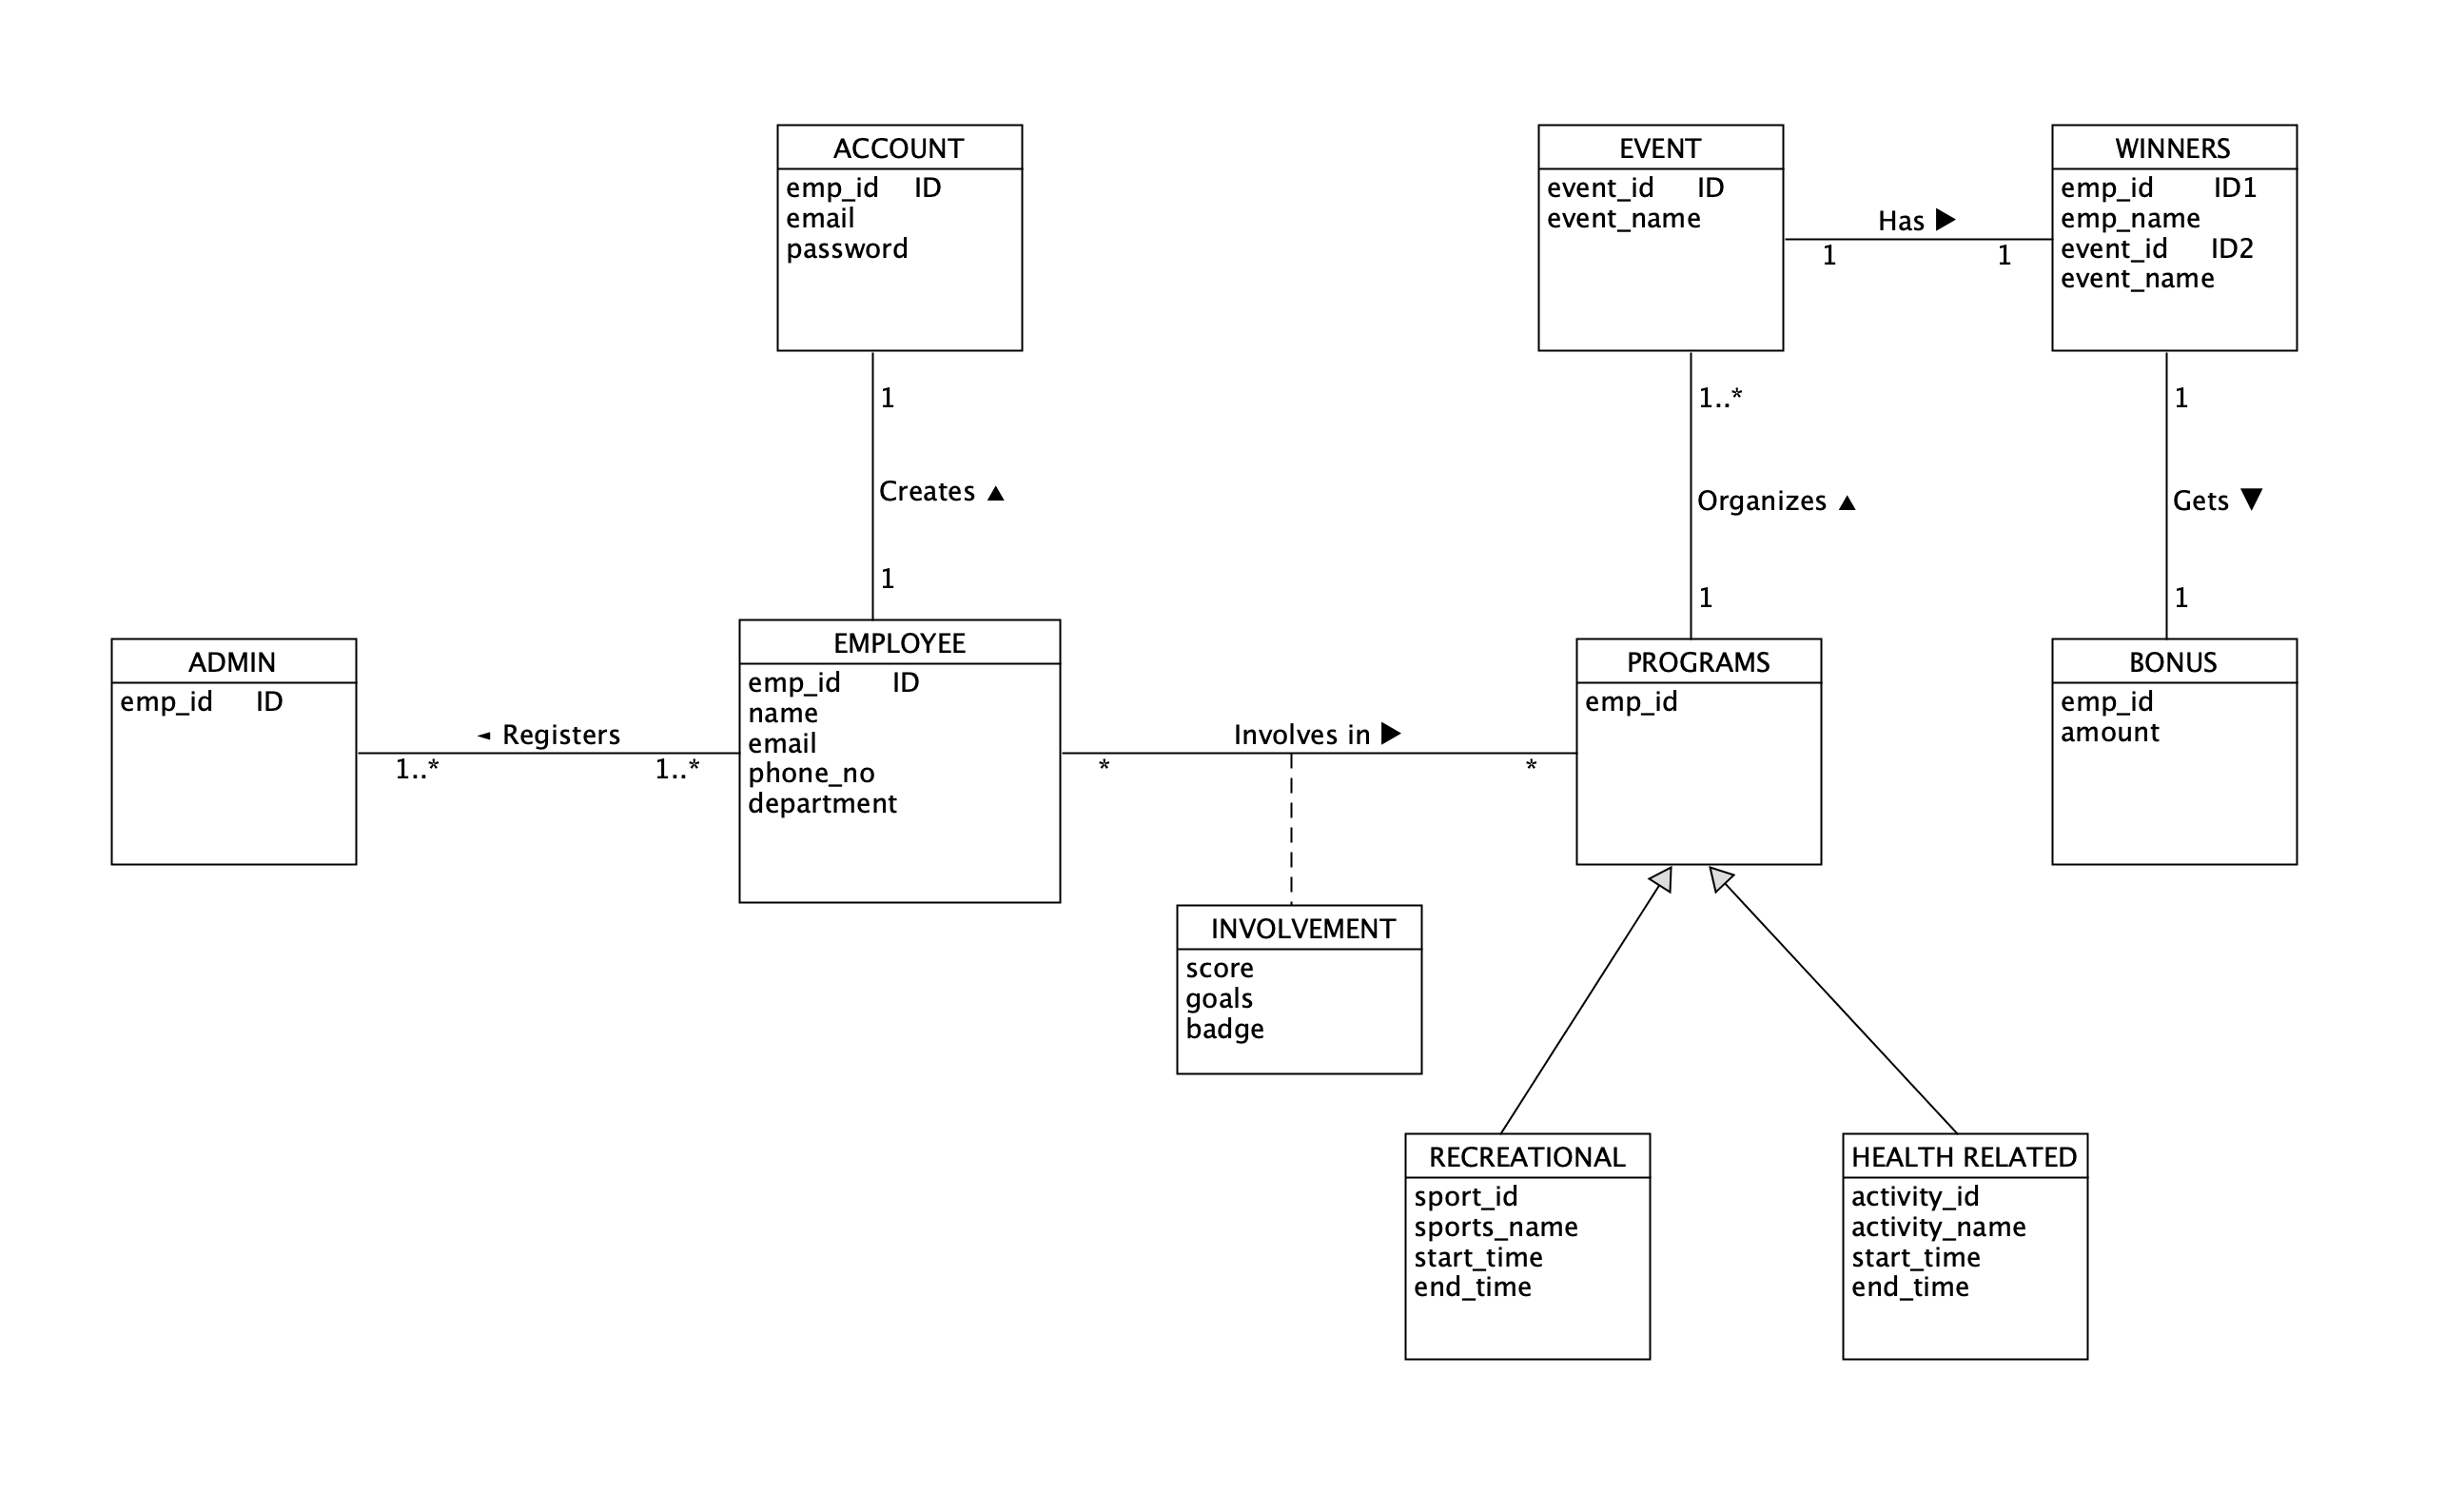
\includegraphics[width=\textwidth]{images/domainClass.png}
    \caption{Domain Class Diagram}
    \label{fig:domainClass}
\end{figure}

\FloatBarrier

\subsection{\textbf{Entities and Attributes:}}
\begin{itemize}
    \item \textbf{ACCOUNT}: Stores account details with attributes \textbf{emp\_id}, \textbf{email} and \textbf{password}.
    \item \textbf{ADMIN}: Represents admin users with attribute \textbf{emp\_id}.
    \item \textbf{EMPLOYEE}: Contains employee details with attributes  \textbf{emp\_id}, \textbf{name}, \textbf{email}, \textbf{phone\_no}, and \textbf{department}.
    \item \textbf{EVENT}: Details of events with attributes \textbf{event\_id} and \textbf{event\_name}.
    \item \textbf{WINNERS}: Keeps track of event winners with attributes \textbf{emp\_id}, \textbf{emp\_name}, \textbf{event\_id}, and \textbf{event\_name}.
    \item \textbf{PROGRAMS}: Holds program details linked to an \textbf{emp\_id}.
    \item \textbf{RECREATIONAL \& HEALTH RELATED}: Subtypes of programs with specific attributes for sports and health activities.
    \item \textbf{BONUS}: Records bonus amounts given to employees with attributes \textbf{emp\_id} and \textbf{amount}.
    \item \textbf{INVOLVEMENT}: Tracks employee involvement in programs with attributes \textbf{score}, \textbf{goals}, and \textbf{badge}. \textbf{INVOLVEMENT} is association class which contains link attributes.
\end{itemize}

\subsection{Relationships}
\begin{itemize}
    \item \textbf{ADMIN} registers multiple \textbf{EMPLOYEEs} (1..* to 1..*).
    \item \textbf{ACCOUNT} is linked to an \textbf{EMPLOYEE} (1 to 1 relationship).
    \item \textbf{EMPLOYEE} creates \textbf{EVENTs} (1 to many relationship).
    \item \textbf{EVENT} organizes \textbf{PROGRAMS} (1 to many relationship).
    \item \textbf{EMPLOYEE} is involved in \textbf{PROGRAMS} (many to many relationship).
    \item \textbf{PROGRAMS} can be either \textbf{RECREATIONAL} or \textbf{HEALTH RELATED} (inheritance relationship).
    \item \textbf{EVENT} has \textbf{WINNERS} (1 to 1 relationship).
    \item \textbf{EMPLOYEE} receives \textbf{BONUS} (1 to 1 relationship).
    
\end{itemize}

\section{Use Case Diagram}

\subsection{Registration Subsystem}
A Use Case Diagram for a Registration Subsystem is shown in the diagram. Use case diagrams, which depict how the system interacts with outside actors, are used to illustrate the functional requirements of a system. 


\begin{table}[h!t]
    \caption{The Registration Subsystem Use Cases}
    {%
    \newcommand{\mc}[2]{\multicolumn{#1}{#2}}
    \begin{center}
    \begin{tabular}{|c|c|}
    \hline
    \multicolumn{2}{|c|}{\textbf{RWIP Registration Subsystem}} \\ \cline{1-2}
    \textbf{Use Cases} & \textbf{Users/Actors} \\
    \hline
    \rule{0pt}{24pt}  Create Account & Employee \\
    \hline
    \rule{0pt}{24pt}  Verify Account & Employee \\
    \hline
    \rule{0pt}{24pt}  Login to Account & Employee \\
    \hline
    \end{tabular}
    \end{center}
    }%
    \label{tab:reg}
\end{table}


\subsubsection{Components of the Use Case Diagram }
\begin{itemize}
    \item \textbf{Actors: }\textbf{Employee} is the primary actor interacting with the Registration Subsystem. Actors are represented by stick figures.
    \item \textbf{System Boundary: }The "Registration Subsystem" rectangle denotes the extent of the system under consideration. Every use case falling under this bound belongs to the Registration Subsystem.
    \item \textbf{Use Cases: }
    \begin{enumerate}
        \item \textbf{Create Account: }This use case represents the process of creating a new account in the system. 
        \item \textbf{Verify Account: }This use case represents the process of verifying an existing account. 
        \item \textbf{Login to Account: } This use case represents the process of logging into an account. 
    \end{enumerate} 
    \item \textbf{Relationships: }Interactions between the actor and the functionalities of the system are shown by lines linking the actor (employee) to each use case (Create Account, Verify Account, and Login to Account). 
\end{itemize}


\begin{figure}[h!t]
    \centering
    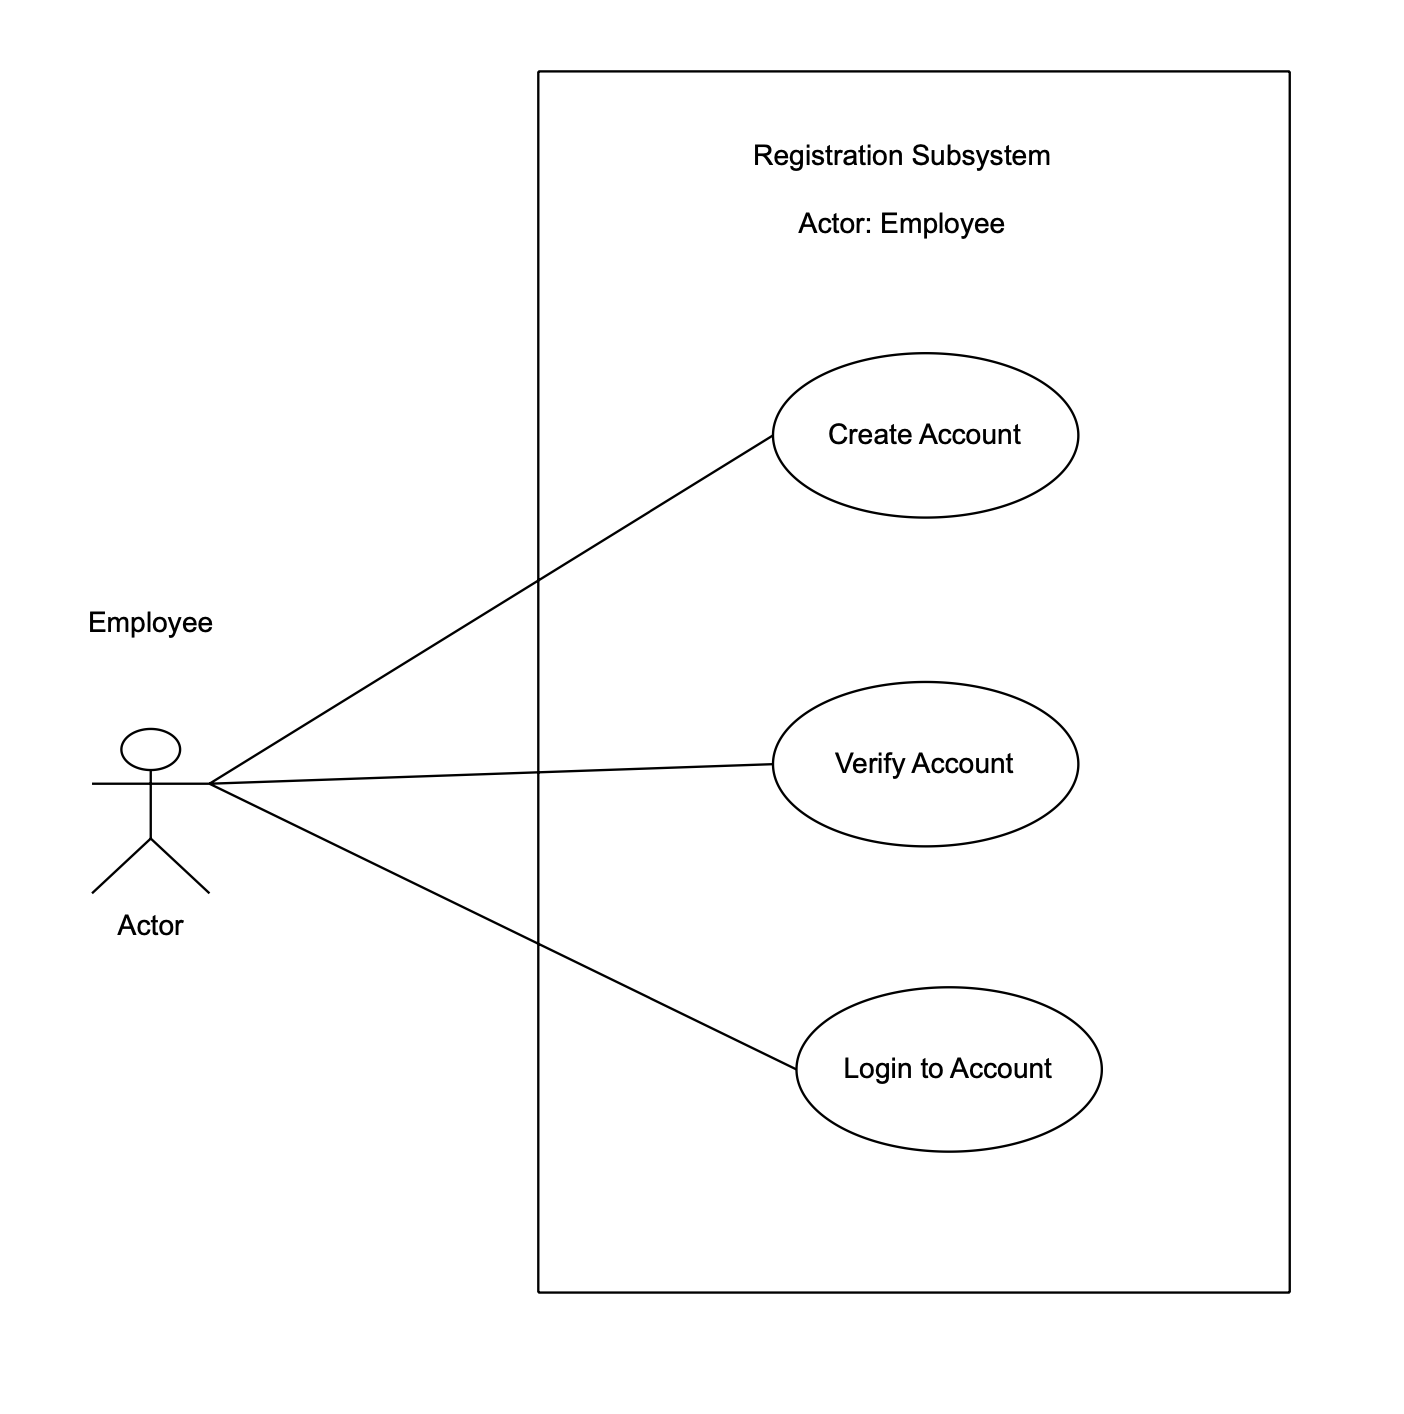
\includegraphics[width=\textwidth]{images/ucRegistration.png}
    \caption{Use case diagram for Registration subsystem}
    \label{fig:ucRegistration}
\end{figure}

\FloatBarrier

An executive summary of the features found in the Registration Subsystem and the ways in which employees can utilise them is given in this diagram. 

\subsection{Program Subsystem}
A Use Case Diagram for a Program Subsystem is shown in the diagram. Use case diagrams illustrate the functions of the system by providing a visual representation of the interactions between external actors and the system.

\begin{table}[h!t]
\caption{The Program Subsystem Use Cases}
{%
\newcommand{\mc}[2]{\multicolumn{#1}{#2}}
\begin{center}
\begin{tabular}{|c|c|}
\hline
\multicolumn{2}{|c|}{\textbf{RWIP Program Subsystem}} \\ \cline{1-2}
\textbf{Use Cases} & \textbf{Users/Actors} \\
\hline
\rule{0pt}{24pt}  Login & Employee \\
\hline
\rule{0pt}{24pt}  Select Programs & Employee \\
\hline
\rule{0pt}{24pt}  Book/Enroll Programs & Employee \\
\hline
\rule{0pt}{24pt}  Participate in Programs & Employee \\
\hline
\rule{0pt}{24pt}  Update badges and rewards & Employee \\
\hline
\end{tabular}
\end{center}
}%
\label{tab:program}
\end{table}

\subsubsection{Components of the Use Case Diagram }
\begin{itemize}
    \item \textbf{Actors: }\textbf{Employee} is the primary actor interacting with the Program Subsystem. Actors are represented by stick figures  and interact with the system's use cases.
    \item \textbf{System Boundary: }The rectangle labeled "Program Subsystem" defines the scope of the system being modeled. All use cases within this boundary are part of the Program Subsystem. 
    \item \textbf{Use Cases: }
    \begin{enumerate}
        \item \textbf{Login to Account: }This use case represents the process of an employee logging into their account. 
        \item \textbf{Select Programs: }This use case involves the employee selecting programs they are interested in.  
        \item \textbf{Book/Enroll Programs: } This use case covers the actions required for booking or enrolling in the selected programs. 
        \item  \textbf{Participate in Programs: } This use case represents the employee's participation in the programs they have enrolled in.
        \item  \textbf{Update Badges and Rewards } This use case involves updating the employee's badges and rewards based on their participation and achievements. 
    \end{enumerate}
    \item \textbf{Relationships: }Interactions between the actor and the features of the system are represented by lines linking the actor (employee) to each use case (Login to Account, Select Programs, Book/Enroll Programs, Participate in Programs, and Update Badges and Rewards). 
\end{itemize}

\begin{figure}[h!t]
    \centering
    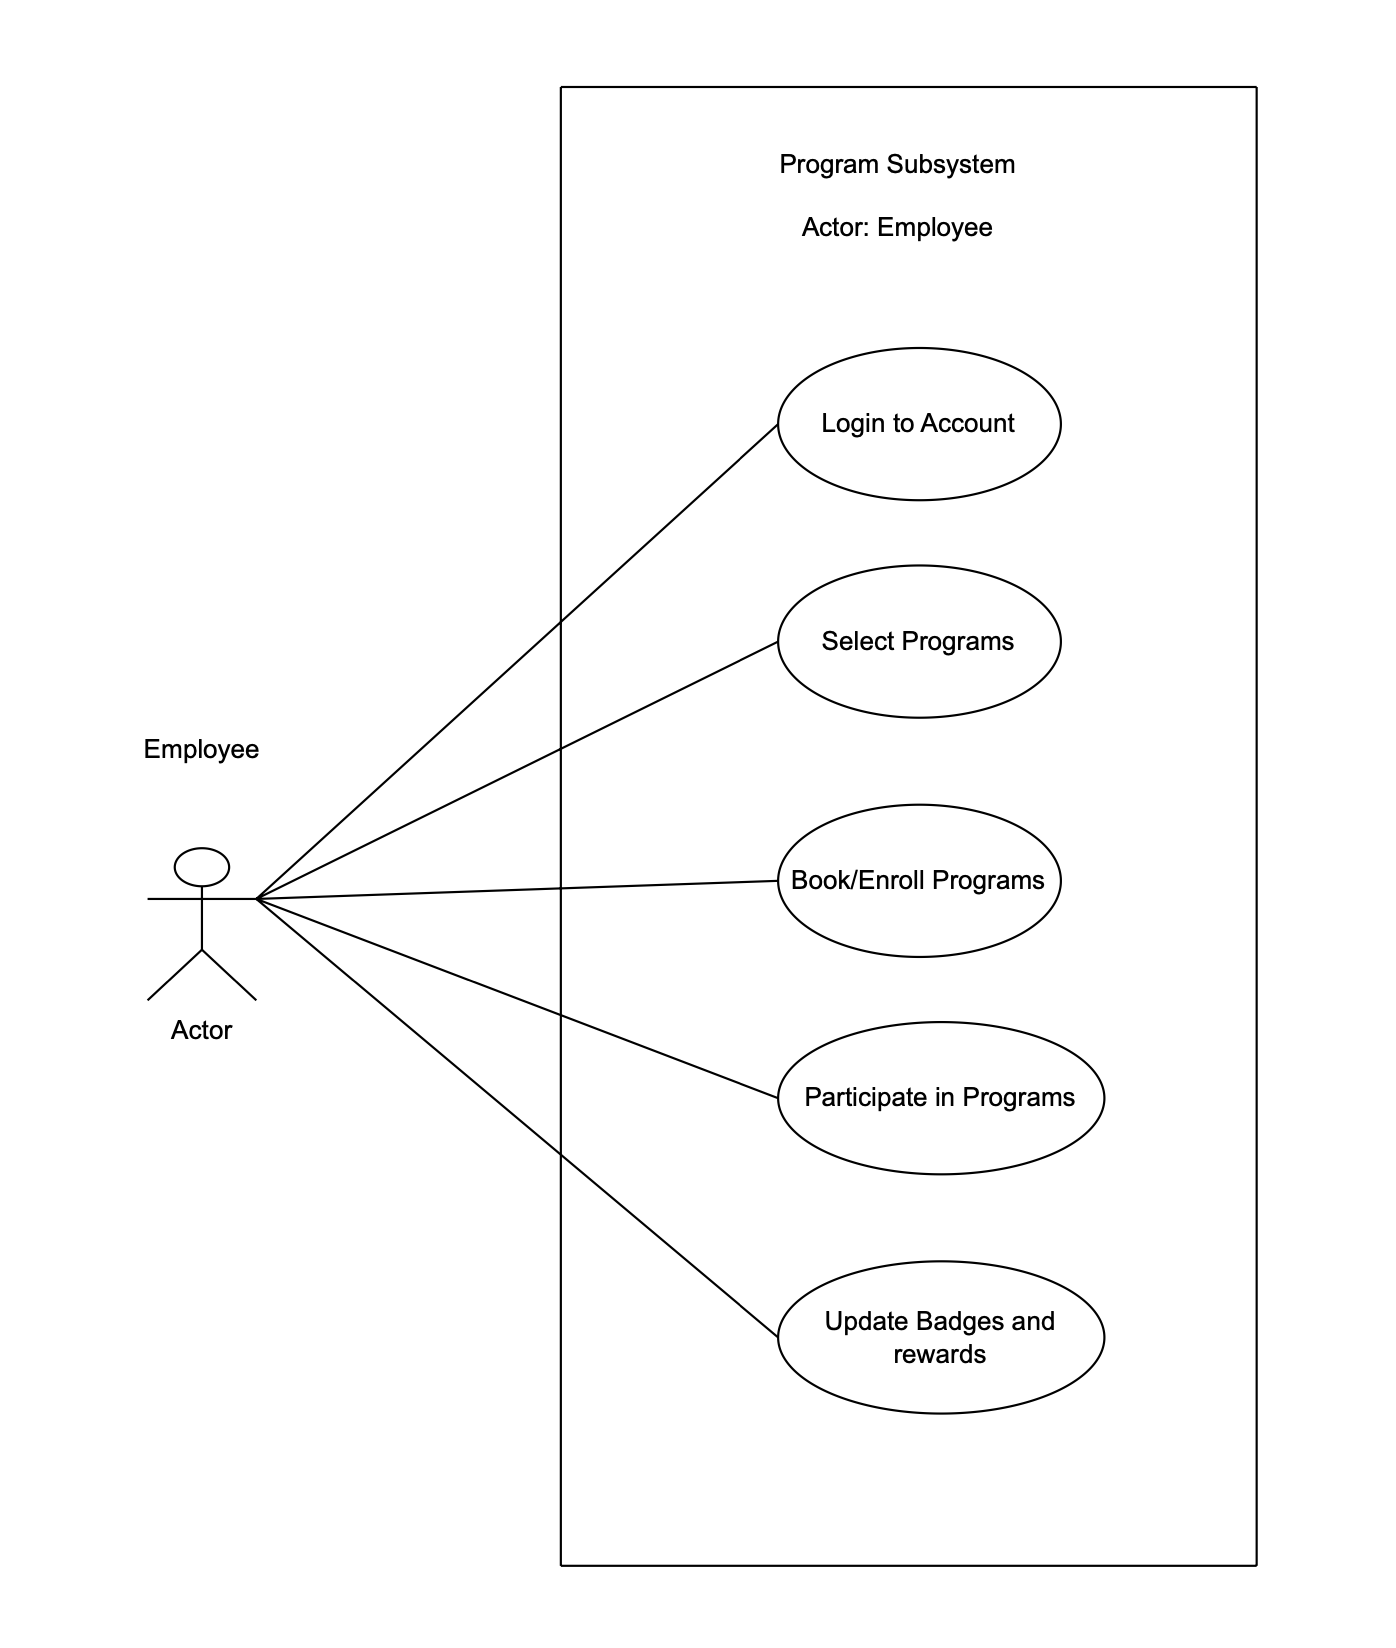
\includegraphics[width=\textwidth]{images/ucProgram.png}
    \caption{Use case diagram for Program subsystem}
    \label{fig:ucProgram}
\end{figure}

\FloatBarrier

This diagram provides a high-level overview of the functionalities available in the Program Subsystem and the interactions that an employee can have with these functionalities. 

\subsection{Event Subsystem}

The provided diagram is a Use Case Diagram for an Event Subsystem. Use case diagrams visually represent the interactions between external actors and the system, highlighting the system's functionalities. 

\begin{table}[h!t]
\caption{The Event Subsystem Use Cases}
{%
\newcommand{\mc}[2]{\multicolumn{#1}{#2}}
\begin{center}
\begin{tabular}{|c|c|}
\hline
\multicolumn{2}{|c|}{\textbf{RWIP Event Subsystem}} \\ \cline{1-2}
\textbf{Use Cases} & \textbf{Users/Actors} \\
\hline
\rule{0pt}{24pt}  Organise Events & HR/Admin \\
\hline
\rule{0pt}{24pt}  Notify Events & HR/Admin, Employee \\
\hline
\rule{0pt}{24pt}  Design Banner & HR/Admin \\
\hline
\rule{0pt}{24pt}  Participate in Events & Employee \\
\hline
\rule{0pt}{24pt}  Declare winners & HR/Admin, Employee \\
\hline
\end{tabular}
\end{center}
}%
\label{tab:event}
\end{table}

\subsubsection{Components of the Use Case Diagram }
\begin{itemize}
    \item \textbf{Actors: }
    \begin{enumerate}
        \item \textbf{HR: }This actor is responsible for managing event-related tasks. Actors are represented by stick figures and interact with the system's use cases. 
        \item \textbf{Employee: }This actor participates in various events and interacts with the system to stay informed and engage in activities. 
    \end{enumerate}
    \item \textbf{System Boundary: }The rectangle labeled "Event Subsystem" defines the scope of the system being modeled. All use cases within this boundary are part of the Event Subsystem. 
    \item \textbf{Use Cases: }
    \begin{enumerate}
        \item \textbf{Organise Events: }This use case represents the process of organizing events. It is primarily associated with the HR actor. 
        \item \textbf{Notify Events: }This use case involves notifying employees about upcoming events. Both HR and employees interact with this functionality. 
        \item \textbf{Design Banne: } This use case covers the creation and design of event banners. It involves both HR and employees.  
        \item  \textbf{Participate in Events: } This use case represents the employee's participation in organized events. 
        \item  \textbf{Declare Winners } This use case involves declaring winners for competitive events. It is managed by HR.
    \end{enumerate}
    \item \textbf{Relationships: } Lines connecting the actors (HR and Employee) to each use case (Organise Events, Notify Events, Design Banner, Participate in Events, and Declare Winners) represent interactions between the actors and the system's functionalities. 
\end{itemize}

\begin{figure}[h!t]
    \centering
    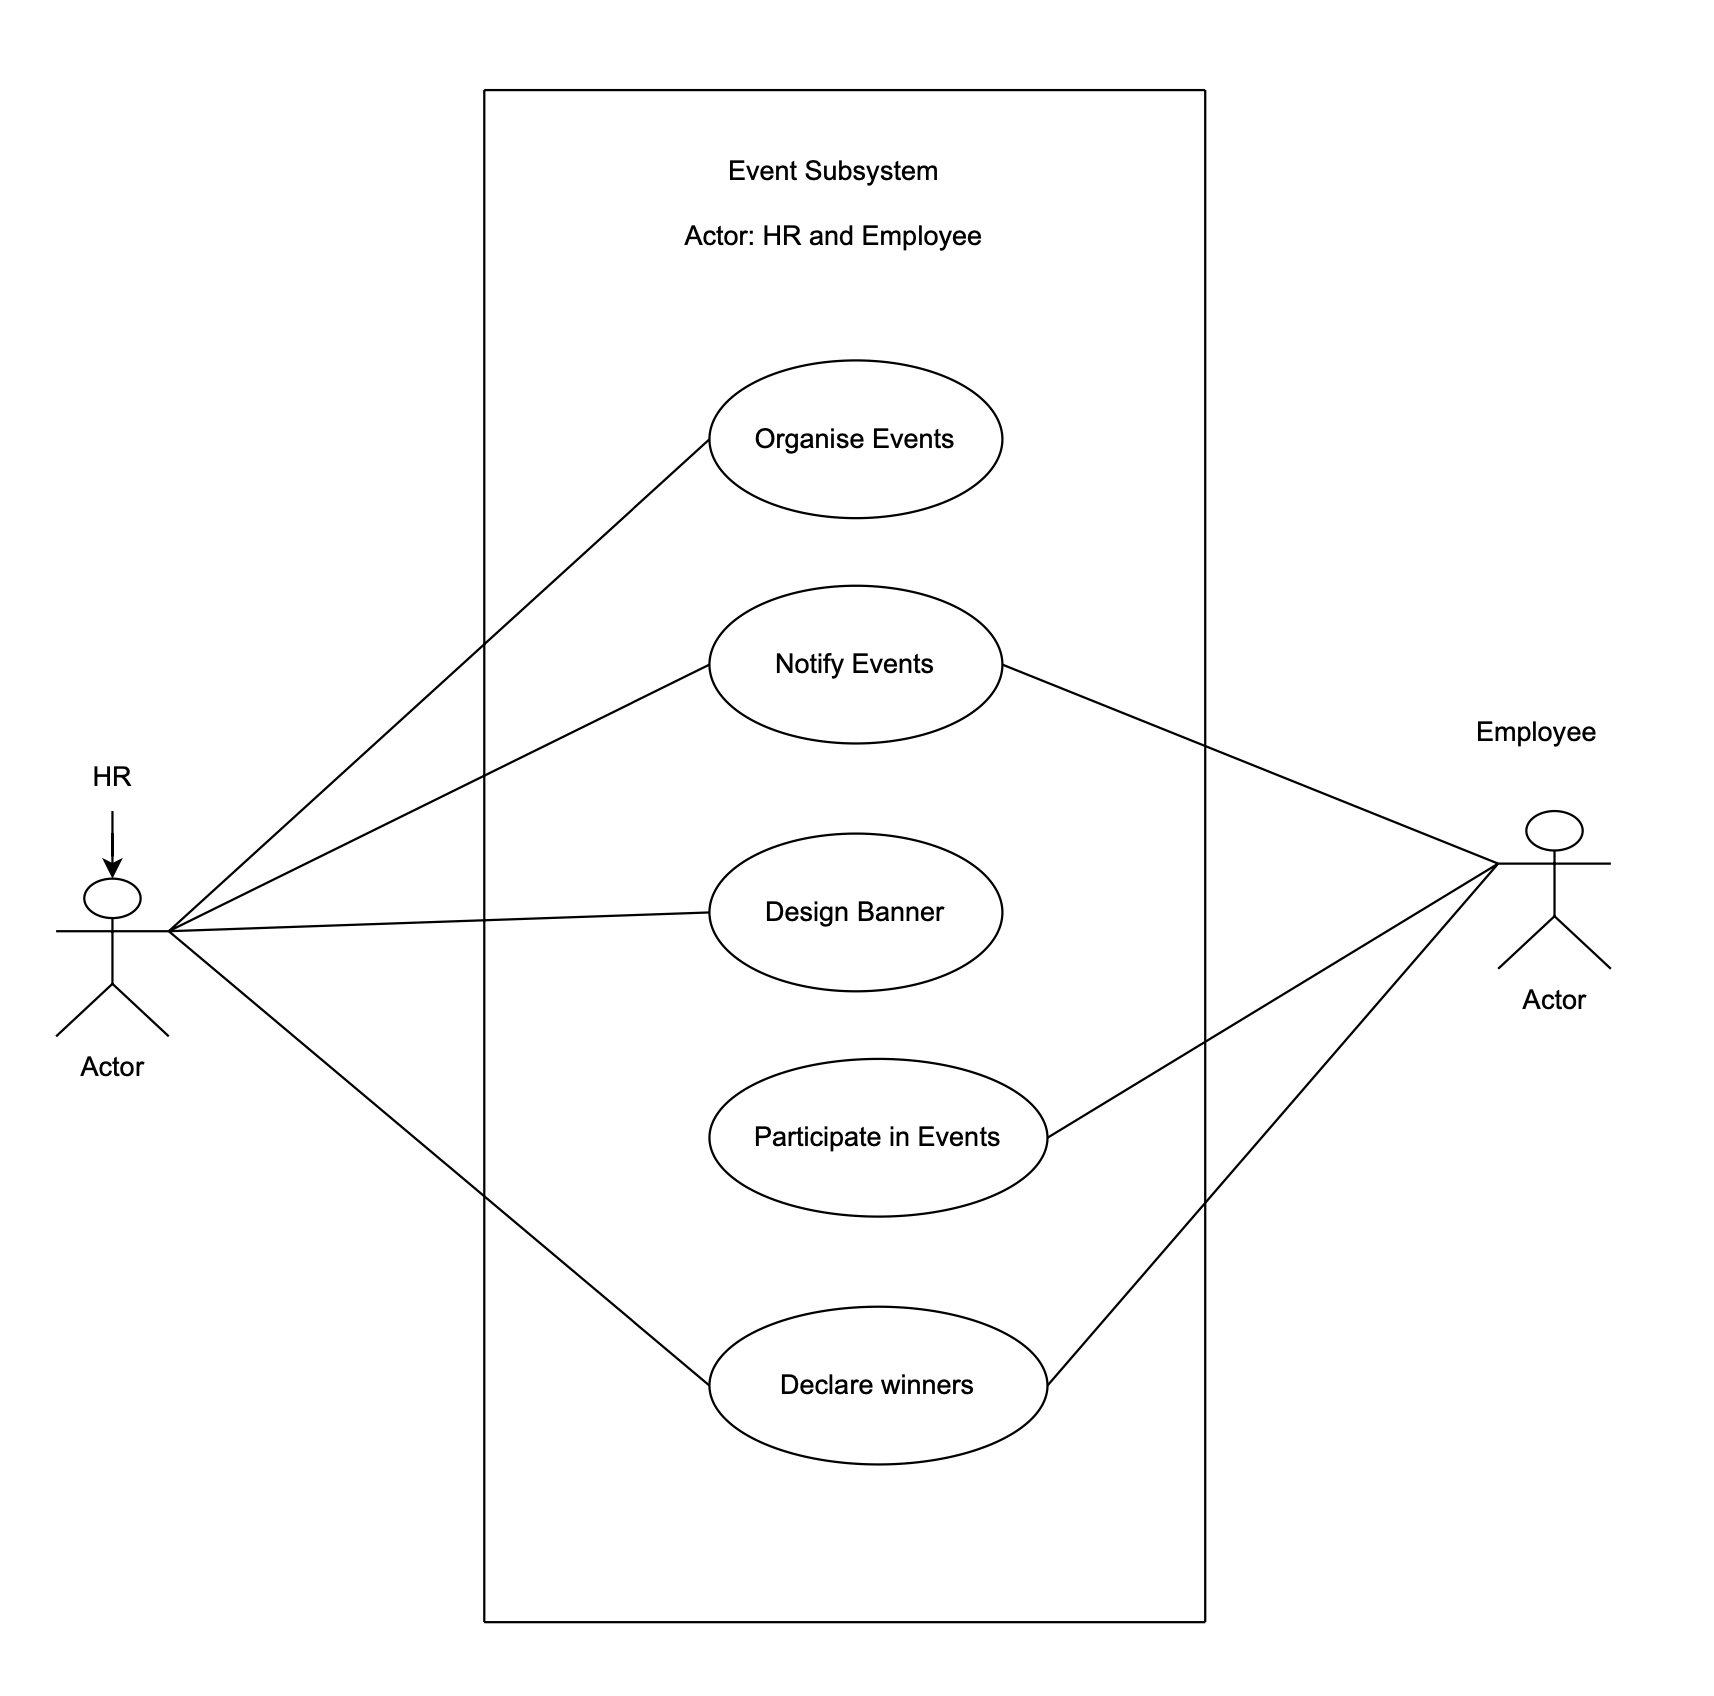
\includegraphics[width=\textwidth]
    {images/ucEvent.png}
    \caption{Use case diagram for Event subsystem}
    \label{fig:ucEvent}
\end{figure}

\FloatBarrier

This diagram provides a high-level overview of the functionalities available in the Event Subsystem and the interactions that HR and employees can have with these functionalities.

\subsection{Payroll Subsystem}
The provided diagram is a Use Case Diagram for a Payroll Subsystem. Use case diagrams visually represent the interactions between external actors and the system, highlighting the system's functionalities. 

\begin{table}[h!t]
\caption{The Payroll Subsystem Use Cases}
{%
\newcommand{\mc}[2]{\multicolumn{#1}{#2}}
\begin{center}
\begin{tabular}{|c|c|}
\hline
\multicolumn{2}{|c|}{\textbf{RWIP Payroll Subsystem}} \\ \cline{1-2}
\textbf{Use Cases} & \textbf{Users/Actors} \\
\hline
\rule{0pt}{24pt} Get the list of winners in different Programs & Payroll Officer, Employee\\
\hline
\rule{0pt}{24pt}  Provide bonuses & Payroll Officer, Employee \\
\hline
\rule{0pt}{24pt}  Update Payroll & Payroll Officer \\
\hline
\end{tabular}
\end{center}
}%
\label{tab:payroll}
\end{table}

\subsubsection{Components of the Use Case Diagram }
\begin{itemize}
    \item \textbf{Actors: }
    \begin{enumerate}
        \item \textbf{Payroll Officer: }This actor is responsible for managing payroll-related tasks, such as getting the list of winners and providing bonuses.  
        \item \textbf{Employee: }This actor participates in events and is eligible to receive bonuses.  
    \end{enumerate}
    \item \textbf{System Boundary: }The rectangle labeled "Payroll Subsystem" defines the scope of the system being modeled. All use cases within this boundary are part of the Payroll Subsystem. 
    \item \textbf{Use Cases: }
    \begin{enumerate}
        \item \textbf{Get List of Winners: }This use case represents the process of obtaining the list of employees who have won awards or competitions. It involves both the Payroll Officer and Employee.  
        \item \textbf{Provide Bonus to Winners: }This use case covers the action of allocating bonuses to employees who are on the winners' list. The Payroll Officer primarily manages this task.   
        \item \textbf{Update Payroll: } This use case involves updating the payroll system to reflect the bonuses provided to the winners. It is managed by the Payroll Officer.  
    \end{enumerate}
    \item \textbf{Relationships: } Lines connecting the actors (Payroll Officer and Employee) to each use case (Get List of Winners, Provide Bonus to Winners, and Update Payroll) represent interactions between the actors and the system's functionalities.  
\end{itemize}

\begin{figure}[h!t]
    \centering
    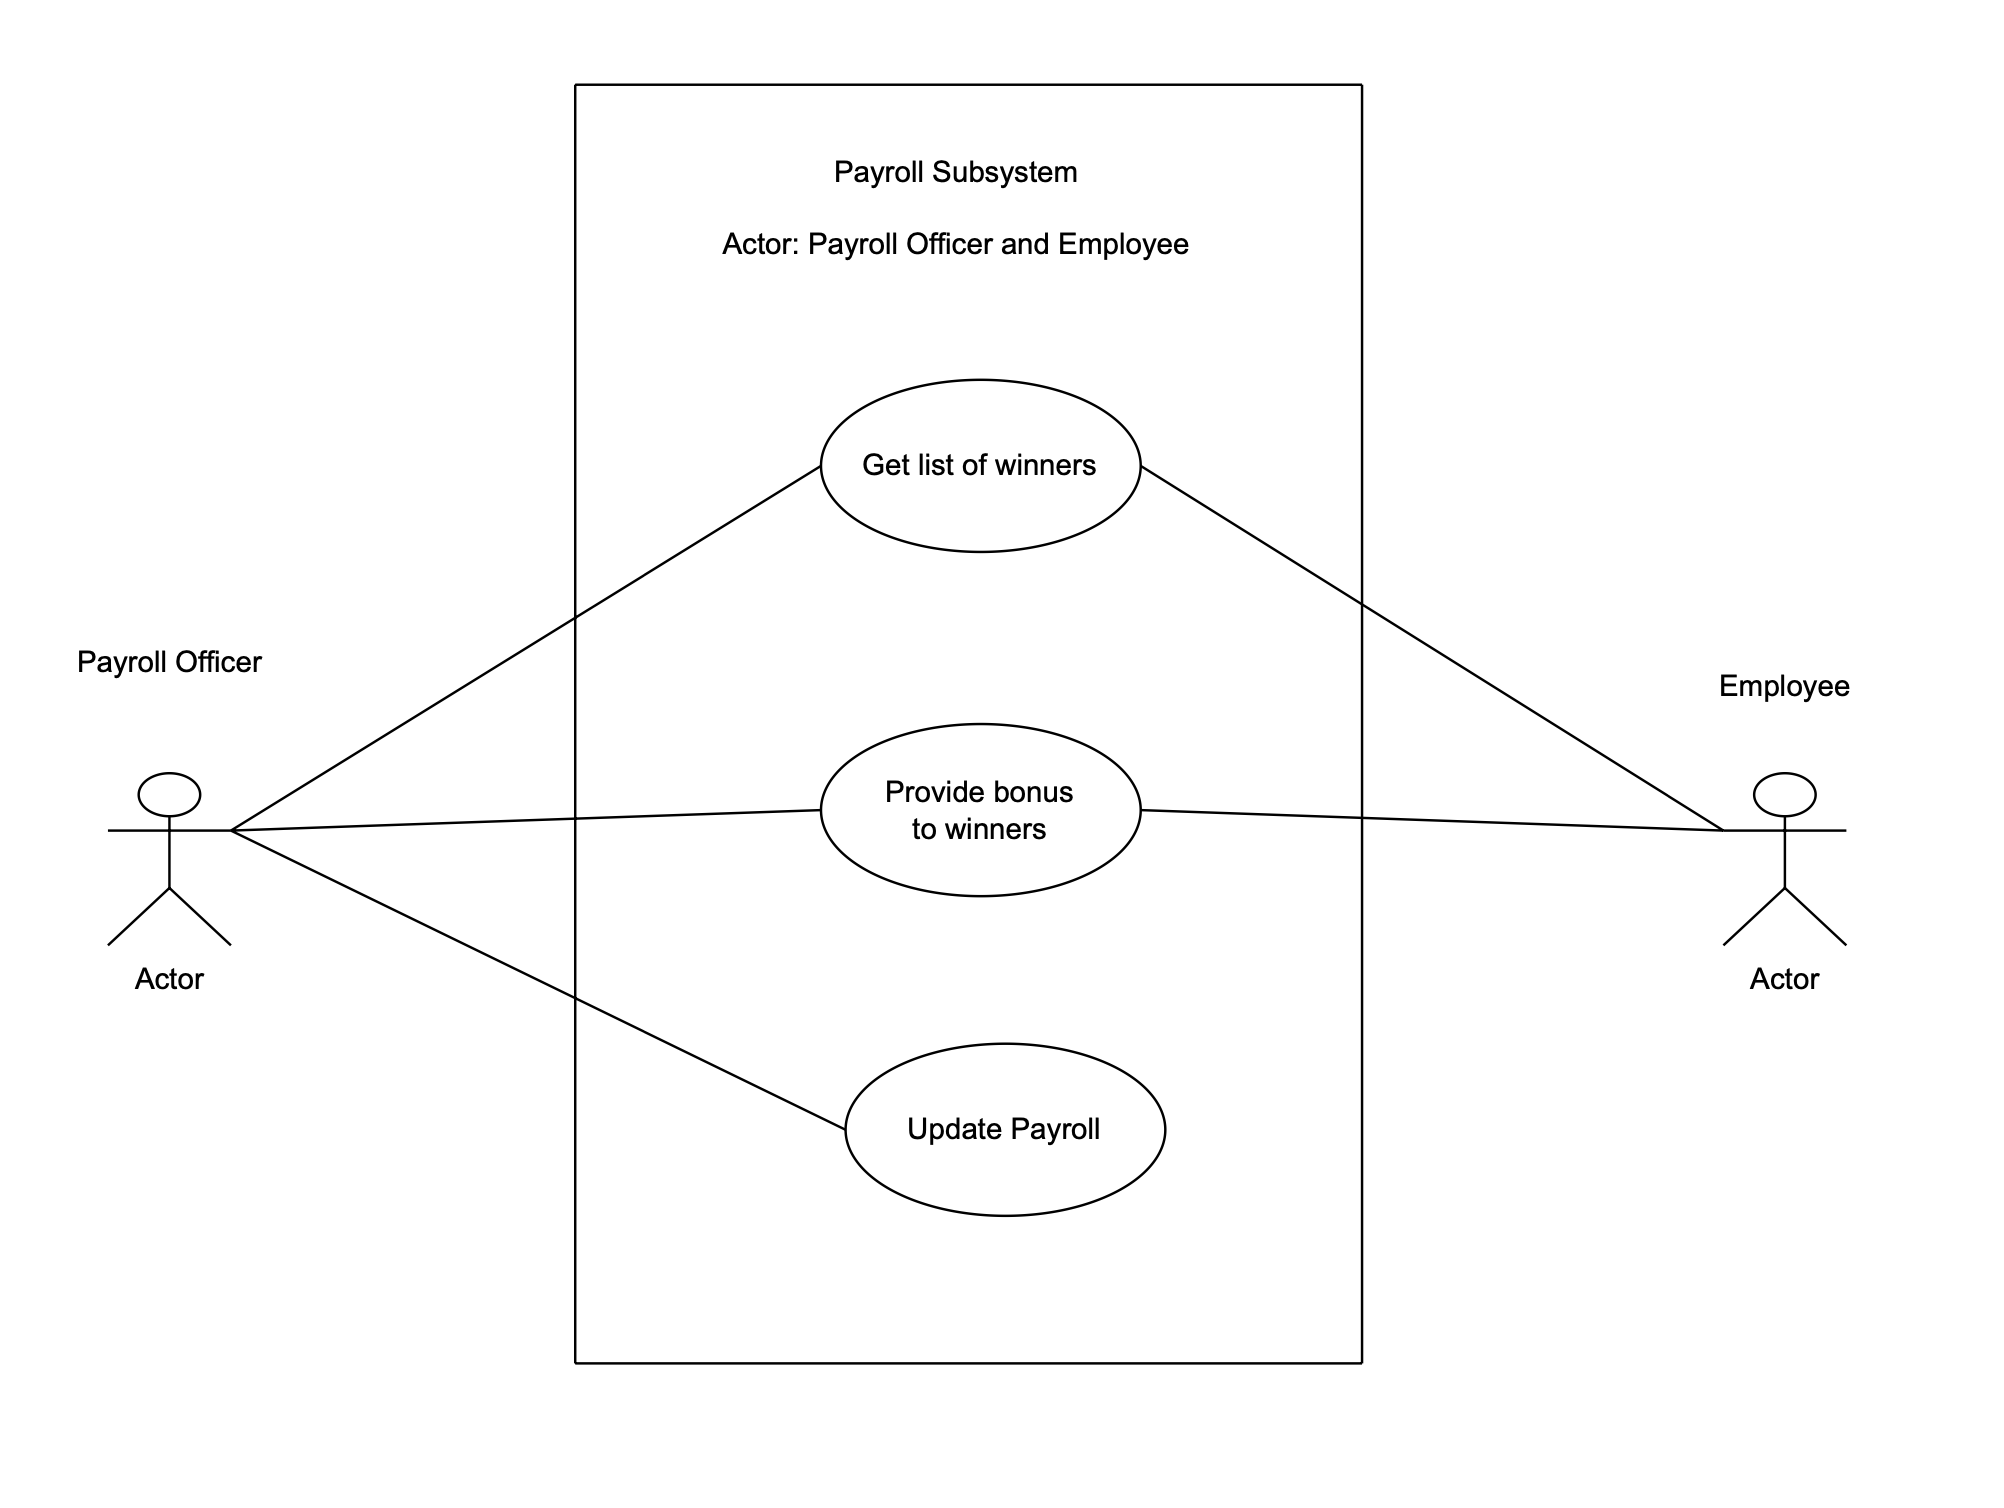
\includegraphics[width=\textwidth]{images/ucPayroll.png}
    \caption{Use case diagram for Payroll subsystem}
    \label{fig:ucPayroll}
\end{figure}

\FloatBarrier

This diagram provides a high-level overview of the functionalities available in the Payroll Subsystem and the interactions that the Payroll Officer and employees can have with these functionalities.

\subsection{Analysis Subsystem}
The provided diagram is a Use Case Diagram for an Analyst Subsystem. Use case diagrams visually represent the interactions between external actors and the system, highlighting the system's functionalities. 

\begin{table}[h!t]
\caption{The Analysis Subsystem Use Cases}
{%
\newcommand{\mc}[2]{\multicolumn{#1}{#2}}
\begin{center}
\begin{tabular}{|c|c|}
\hline
\multicolumn{2}{|c|}{\textbf{RWIP Analysis Subsystem}} \\ \cline{1-2}
\textbf{Use Cases} & \textbf{Users/Actors} \\
\hline
\rule{0pt}{24pt}  Register as Admin & Analyst \\
\hline
\rule{0pt}{24pt}  Login as Admin & Analyst \\
\hline
\rule{0pt}{24pt}  Fetch Data & Analyst \\
\hline
\rule{0pt}{24pt}  Analyze Data & Analyst \\
\hline
\rule{0pt}{24pt}  Generate Report & Analyst, Developers \\
\hline
\rule{0pt}{24pt}  Make Decisions & Analyst \\
\hline
\end{tabular}
\end{center}
}%
\label{tab:analysis}
\end{table}

\subsubsection{Components of the Use Case Diagram }
\begin{itemize}
    \item \textbf{Actors: }
    \begin{enumerate}
        \item \textbf{Analyst: }This actor is responsible for data analysis and decision-making tasks. 
        \item \textbf{Developer: }This actor interacts with the system to perform specific tasks related to data fetching and analysis support. 
    \end{enumerate}
    \item \textbf{System Boundary: }The rectangle labeled "Analyst Subsystem" defines the scope of the system being modeled. All use cases within this boundary are part of the Analyst Subsystem. 
    \item \textbf{Use Cases: }
    \begin{enumerate}
        \item \textbf{Register as Admin: }This use case represents the process of an analyst registering as an admin within the system. 
        \item \textbf{Login as Admin: }This use case covers the action of logging in as an admin to access system functionalities.   
        \item \textbf{Fetch Data: } This use case involves retrieving necessary data for analysis. Both the analyst and the developer can interact with this functionality. 
        \item  \textbf{Analyze Data: } This use case represents the process of analyzing the retrieved data. It is primarily performed by the analyst. 
        \item  \textbf{Generate Reports } This use case covers the creation of reports based on the analyzed data.  
        \item  \textbf{Make Decisions } This use case involves making decisions based on the generated reports and analyzed data.
    \end{enumerate}
    \item \textbf{Relationships: }Lines connecting the actors (Analyst and Developer) to each use case (Register as Admin, Login as Admin, Fetch Data, Analyze Data, Generate Reports, and Make Decisions) represent interactions between the actors and the system's functionalities. 
\end{itemize}

\begin{figure}[h!t]
    \centering
    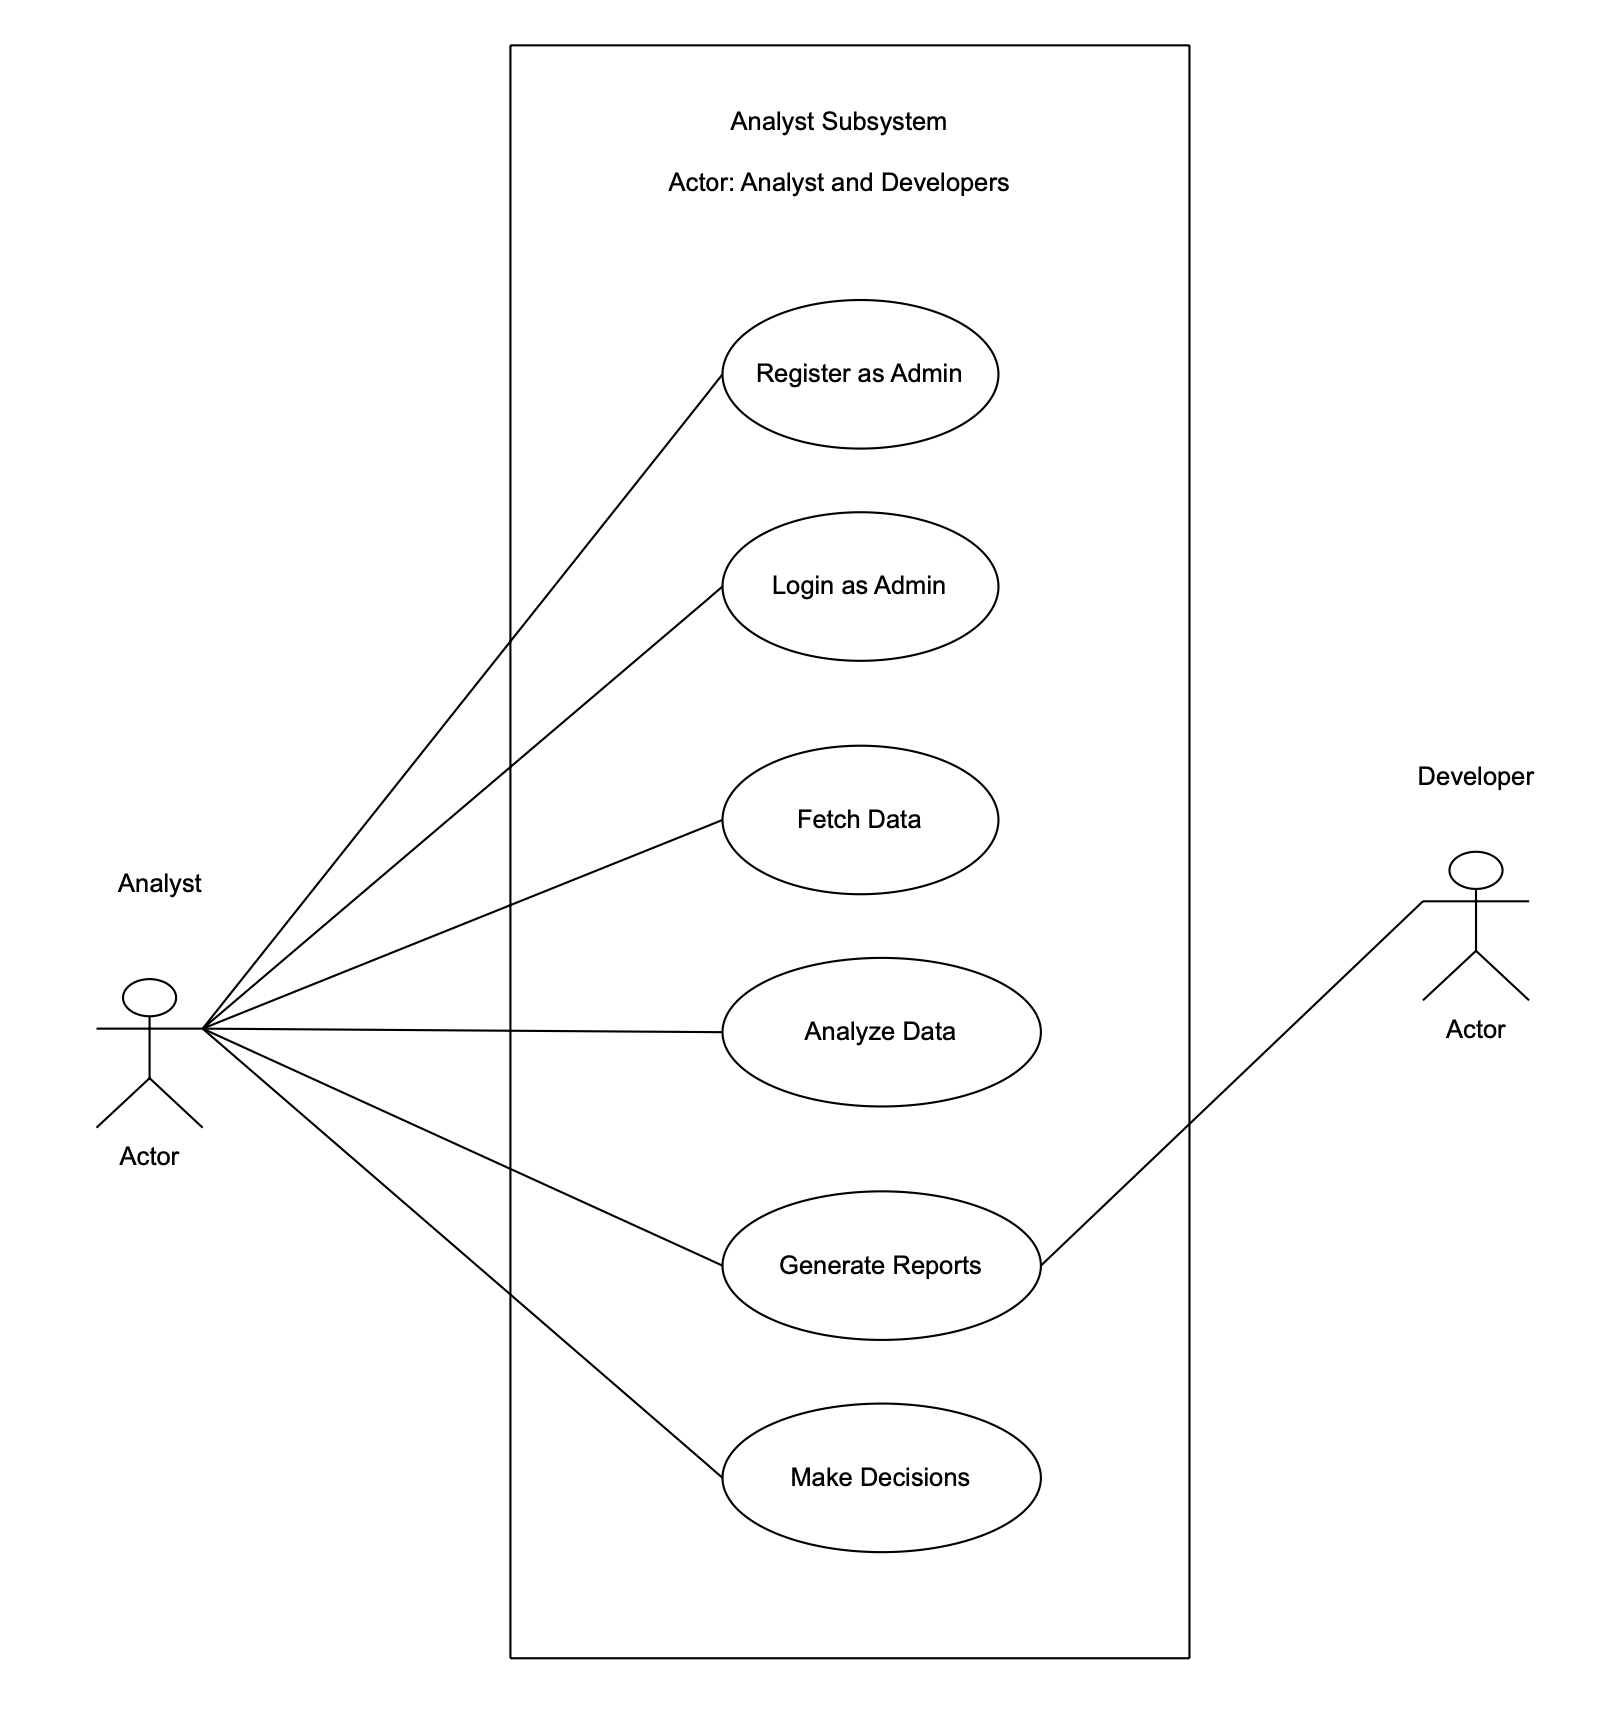
\includegraphics[width=\textwidth]{images/ucAnaysis.png}
    \caption{Use case diagram for Analysis subsystem}
    \label{fig:ucAnaysis}
\end{figure}

\FloatBarrier

This diagram provides a high-level overview of the functionalities available in the Analyst Subsystem and the interactions that analysts and developers can have with these functionalities. 

\section{Fully Developed Use Case Description}

\begin{table}[h!t]
    \caption{Register/Create Account}
    \begin{center}
    \small % Set font size to small
    \begin{tabularx}{\textwidth}{|l|X|}
    \hline
    \rule{0pt}{24pt}  \textbf{Use case name:} & Create employee account \\
    \hline
    \rule{0pt}{24pt}  \textbf{Scenario:} & Create online employee account \\
    \hline
    \rule{0pt}{24pt}  \textbf{Triggering event:} & Employee wants to join the recreational and wellness programs \\
    \hline
    \rule{0pt}{24pt}  \textbf{Brief description:} & Employee signs up or creates new account by providing their employee email id to access, book and participate in activity \\
    \hline
    \rule{0pt}{24pt}  \textbf{Actors:} & Employees \\
    \hline
    \rule{0pt}{24pt}  \textbf{Related use cases:} & Admin can create account on behalf of employee \\
    \hline
    \rule{0pt}{24pt}  \textbf{Stakeholders:} & Admin, HR \\
    \hline
    \rule{0pt}{24pt}  \textbf{Pre-conditions:} & Registration subsystem must be available \\
    % Employees must have employer's provided email_id \\
    % Employees must verify the account by clicking on verify link sent on the email
    \hline
    \rule{0pt}{24pt}  \textbf{Post-conditions:} & Employee account must be created and saved \\
    % All the activity must be tracked like badge, rewards received.
    \hline
    \rule{0pt}{24pt}  \textbf{Exception conditions:} & Employee might not have email id provided by employer \\
    % Employee have not verified the account by clicking on verification link sent on the mail.
    % Email_id provided is invalid
    \hline
    \end{tabularx}
    \end{center}
    \label{tab:createAccount}
    \end{table}
\FloatBarrier

\section{Sequence Diagram}
The provided diagram is a Sequence Diagram that illustrates the interactions between different components of a system for specific use cases. Sequence diagrams are used to depict the flow of messages, events, and actions between objects or components over time. 
\\
The sequence diagram is divided into four lifelines representing the different components involved in the interactions: Employee, UI, Logic, and Database. 
\begin{figure}[h!t]
    \centering
    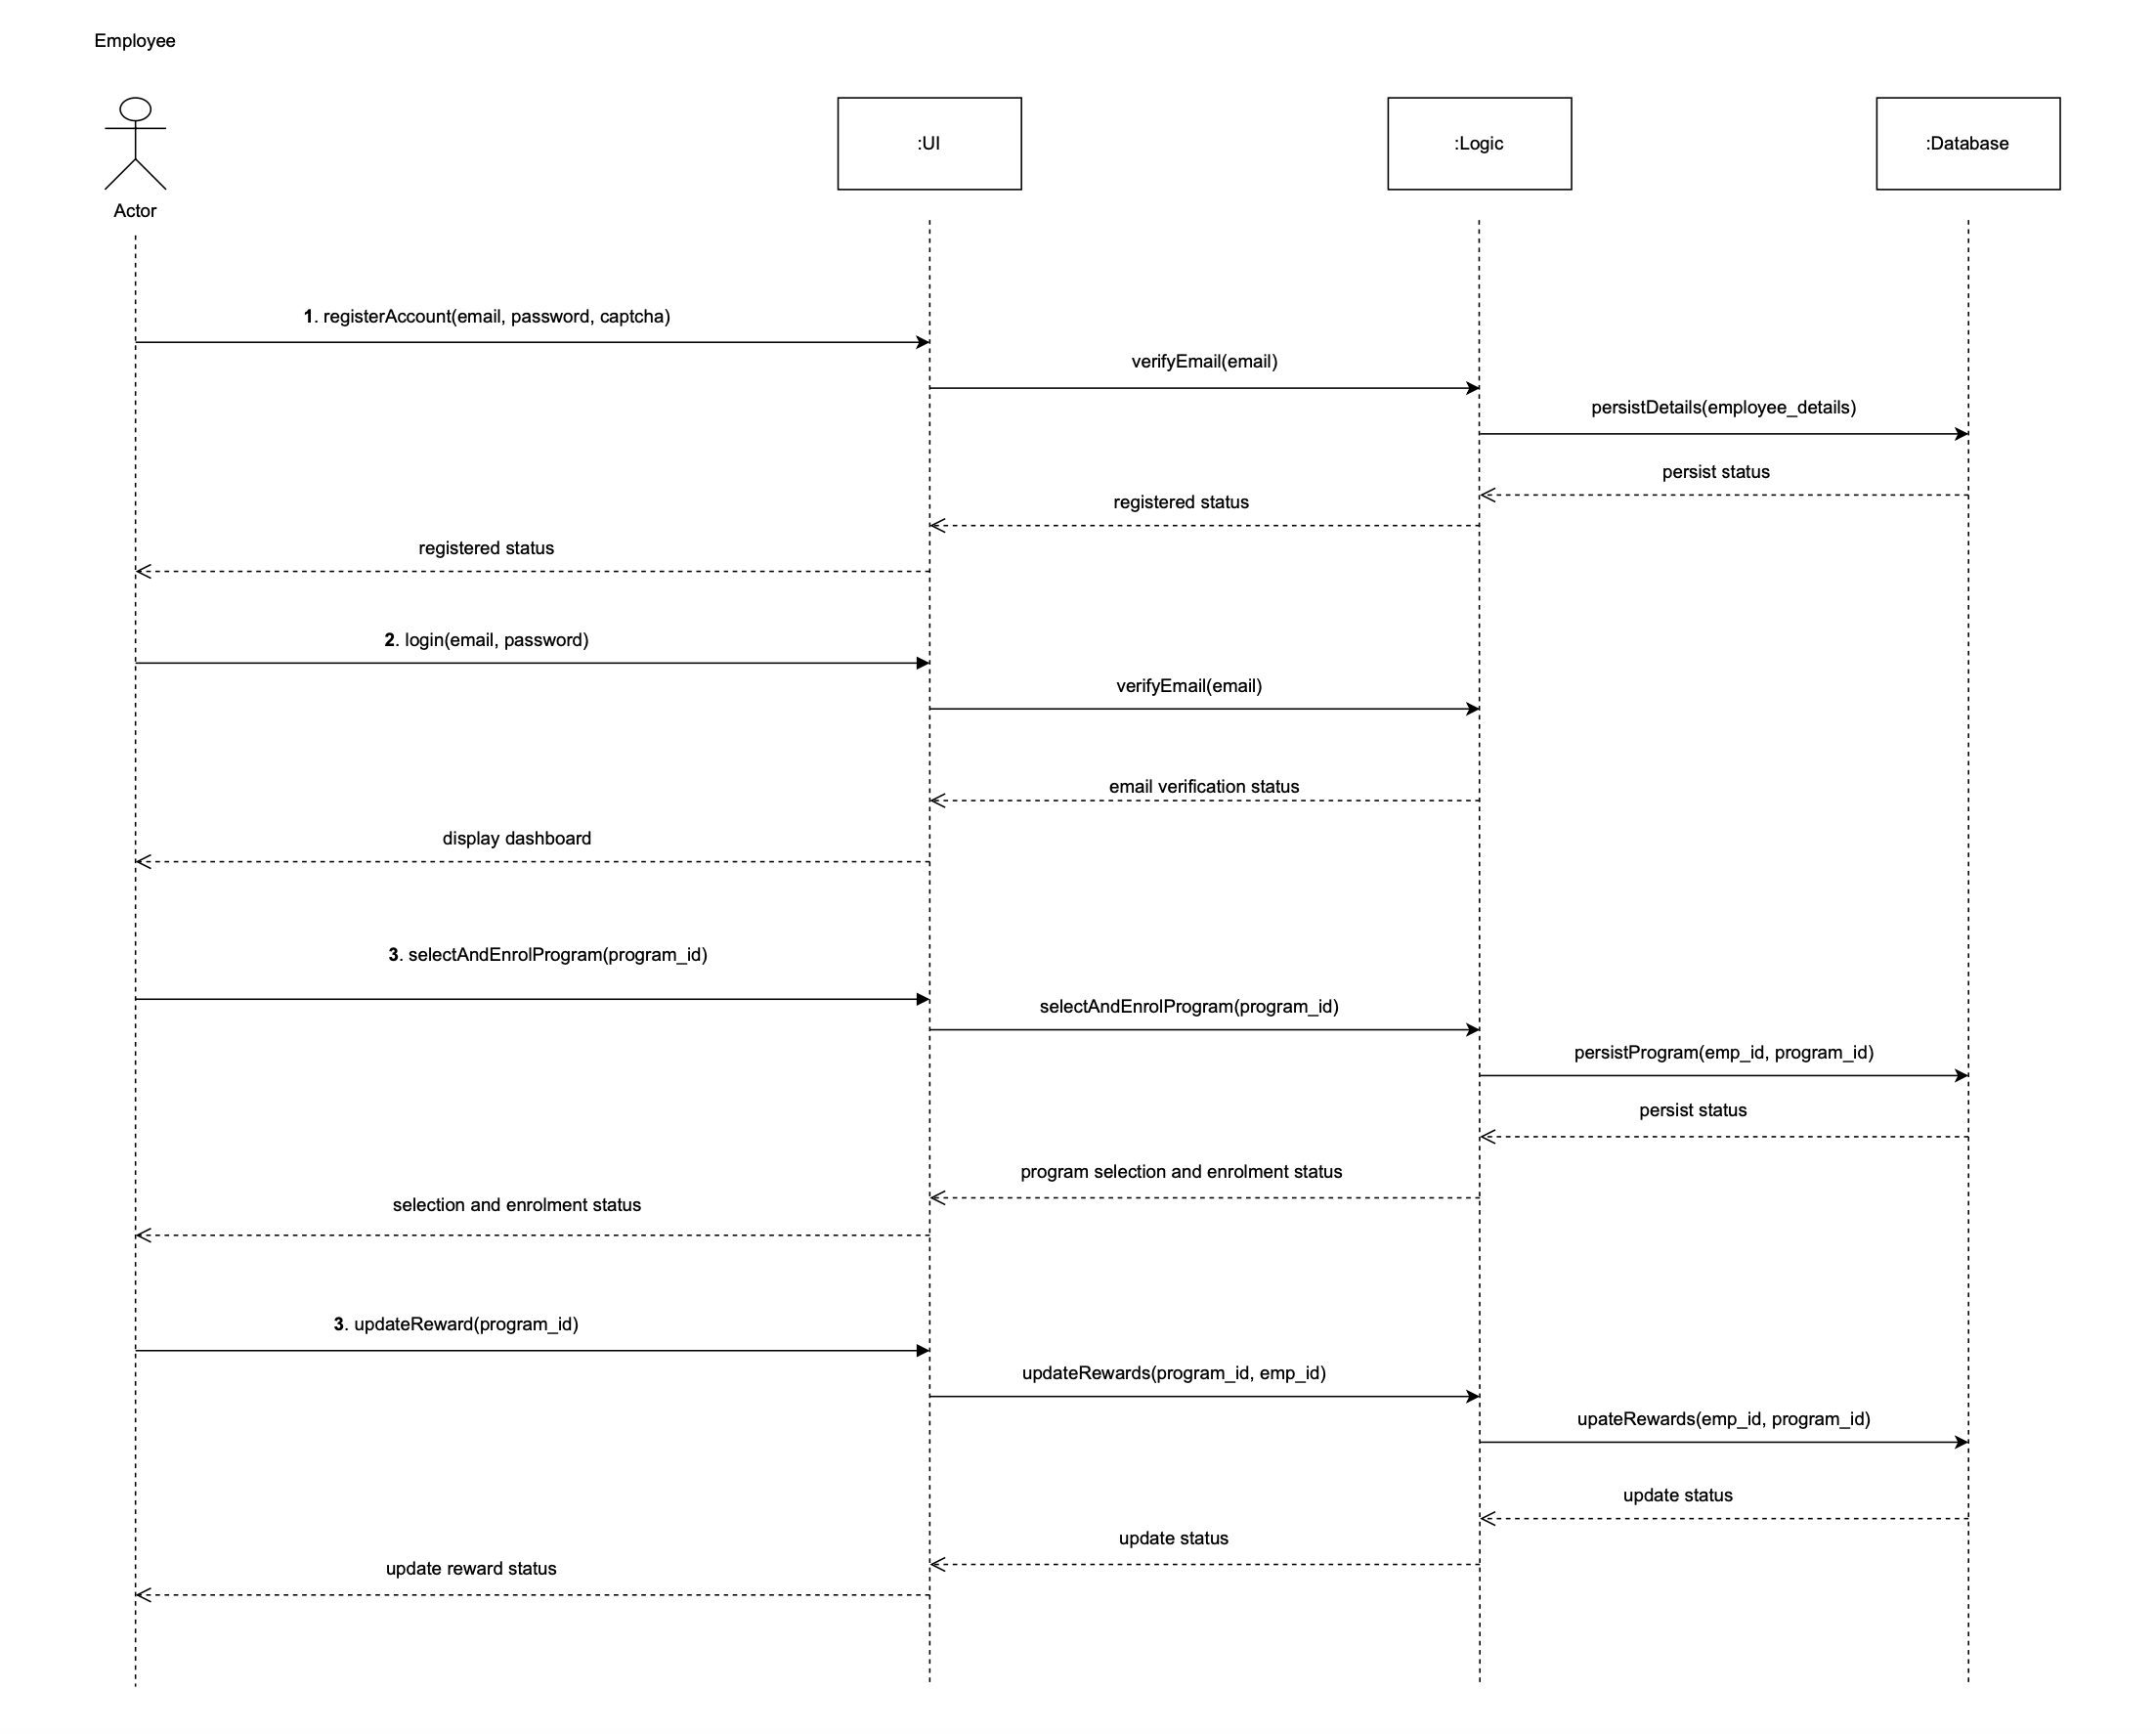
\includegraphics[width=\textwidth]{images/sequenceDiagram.png}
    \caption{Sequence Diagram}
    \label{fig:sequenceDiagram}
\end{figure}

\FloatBarrier


\subsection{Details of Interactions}
\textbf{Register Account}
\begin{itemize}
    \item Employee initiates the process by calling registerAccount(email, password, captcha) on the UI. 
    \item UI forwards the verifyEmail(email) request to Logic. 
    \item Logic processes the email verification and responds with registered status to UI. 
    \item UI then sends persistDetails(employee\_details) to the Database to save the registration details. 
    \item Database returns persist status to Logic, which is then propagated back to the UI. 
\end{itemize}
\leavevmode
\newline
\textbf{Register Account}
\begin{itemize}
    \item Employee sends login(email, password) to the UI. 
    \item UI forwards the verifyEmail(email) request to Logic for email verification.
    \item Logic processes the verification and returns email verification status to UI. 
    \item If the verification is successful, UI displays the dashboard to the employee.
\end{itemize}
\leavevmode
\newline
\textbf{Select and Enroll in Program }
\begin{itemize}
    \item Employee initiates program selection by calling selectAndEnrollProgram(program\_id) on the UI. 
    \item UI sends the selectAndEnrollProgram(program\_id) request to Logic. 
    \item Logic processes the program selection and sends persistProgram(emp\_id, program\_id) to the Database to save the enrollment details.
    \item Database returns persist status to Logic, which then returns program selection and enrollment status to UI. 
\end{itemize}
\leavevmode
\newline
\textbf{Update Reward }
\begin{itemize}
    \item Employee calls updateReward(program\_id) on the UI to update rewards based on program participation. 
    \item UI forwards the updateRewards(program\_id, emp\_id) request to Logic. 
    \item Logic processes the reward update and sends updateRewards(emp\_id, program\_id) to the Database to save the updated reward details. 
    \item Database returns update status to Logic, which then propagates the update status back to UI. 
\end{itemize}

This sequence diagram provides a comprehensive view of the interactions and message exchanges between the employee, UI, logic, and database components for the registration, login, program enrollment, and reward update processes. It clearly shows the flow of control and data, helping to understand the sequence of operations and the dependencies between various system components. 

\section{Activity Diagram}
The provided diagram is an Activity Diagram that illustrates the sequence of activities across various subsystems within a system. Activity diagrams are used to model the workflow of a system and show the flow of control from one activity to another. 
\\
The diagram is divided into five subsystems, each with specific activities and flow of control. 
\leavevmode
\newline
\textbf{Registration Subsystem }
\begin{itemize}
    \item \textbf{Start: }The process begins with the "Start" node. 
    \item \textbf{Employee Registration: }The first activity where an employee registers into the system.
    \item \textbf{Login: }After registration, the employee logs into the system. This activity also connects to the Program Subsystem. 
\end{itemize}
\leavevmode
\newline
\textbf{Programs  Subsystem }
\begin{itemize}
    \item \textbf{Select Programs: }Employees select programs they are interested in.  
    \item \textbf{Enroll/Book Programs: }After selecting, employees enroll or book these programs. 
    \item \textbf{Participate in Programs: }Employees participate in the programs they have enrolled in.  
    \item \textbf{Achieve Goals/Badge: }Participation leads to achieving goals or badges. 
\end{itemize}
\leavevmode
\newline
\textbf{Analysis Subsystem }
\begin{itemize}
    \item \textbf{Register as Admin: }An analyst registers as an admin in the system.
    \item \textbf{Login as Admin: }The analyst logs in as an admin. 
    \item \textbf{Fetch Data: }Data is retrieved for analysis. 
    \item \textbf{Analyze Data: }The fetched data is analyzed.
    \item \textbf{Generate Reports: }Reports are generated based on the analysis, particularly focusing on employee involvement.
    \item \textbf{Make Decisions: }Decisions are made based on the generated reports. 
\end{itemize}

\begin{figure}[h!t]
    \centering
    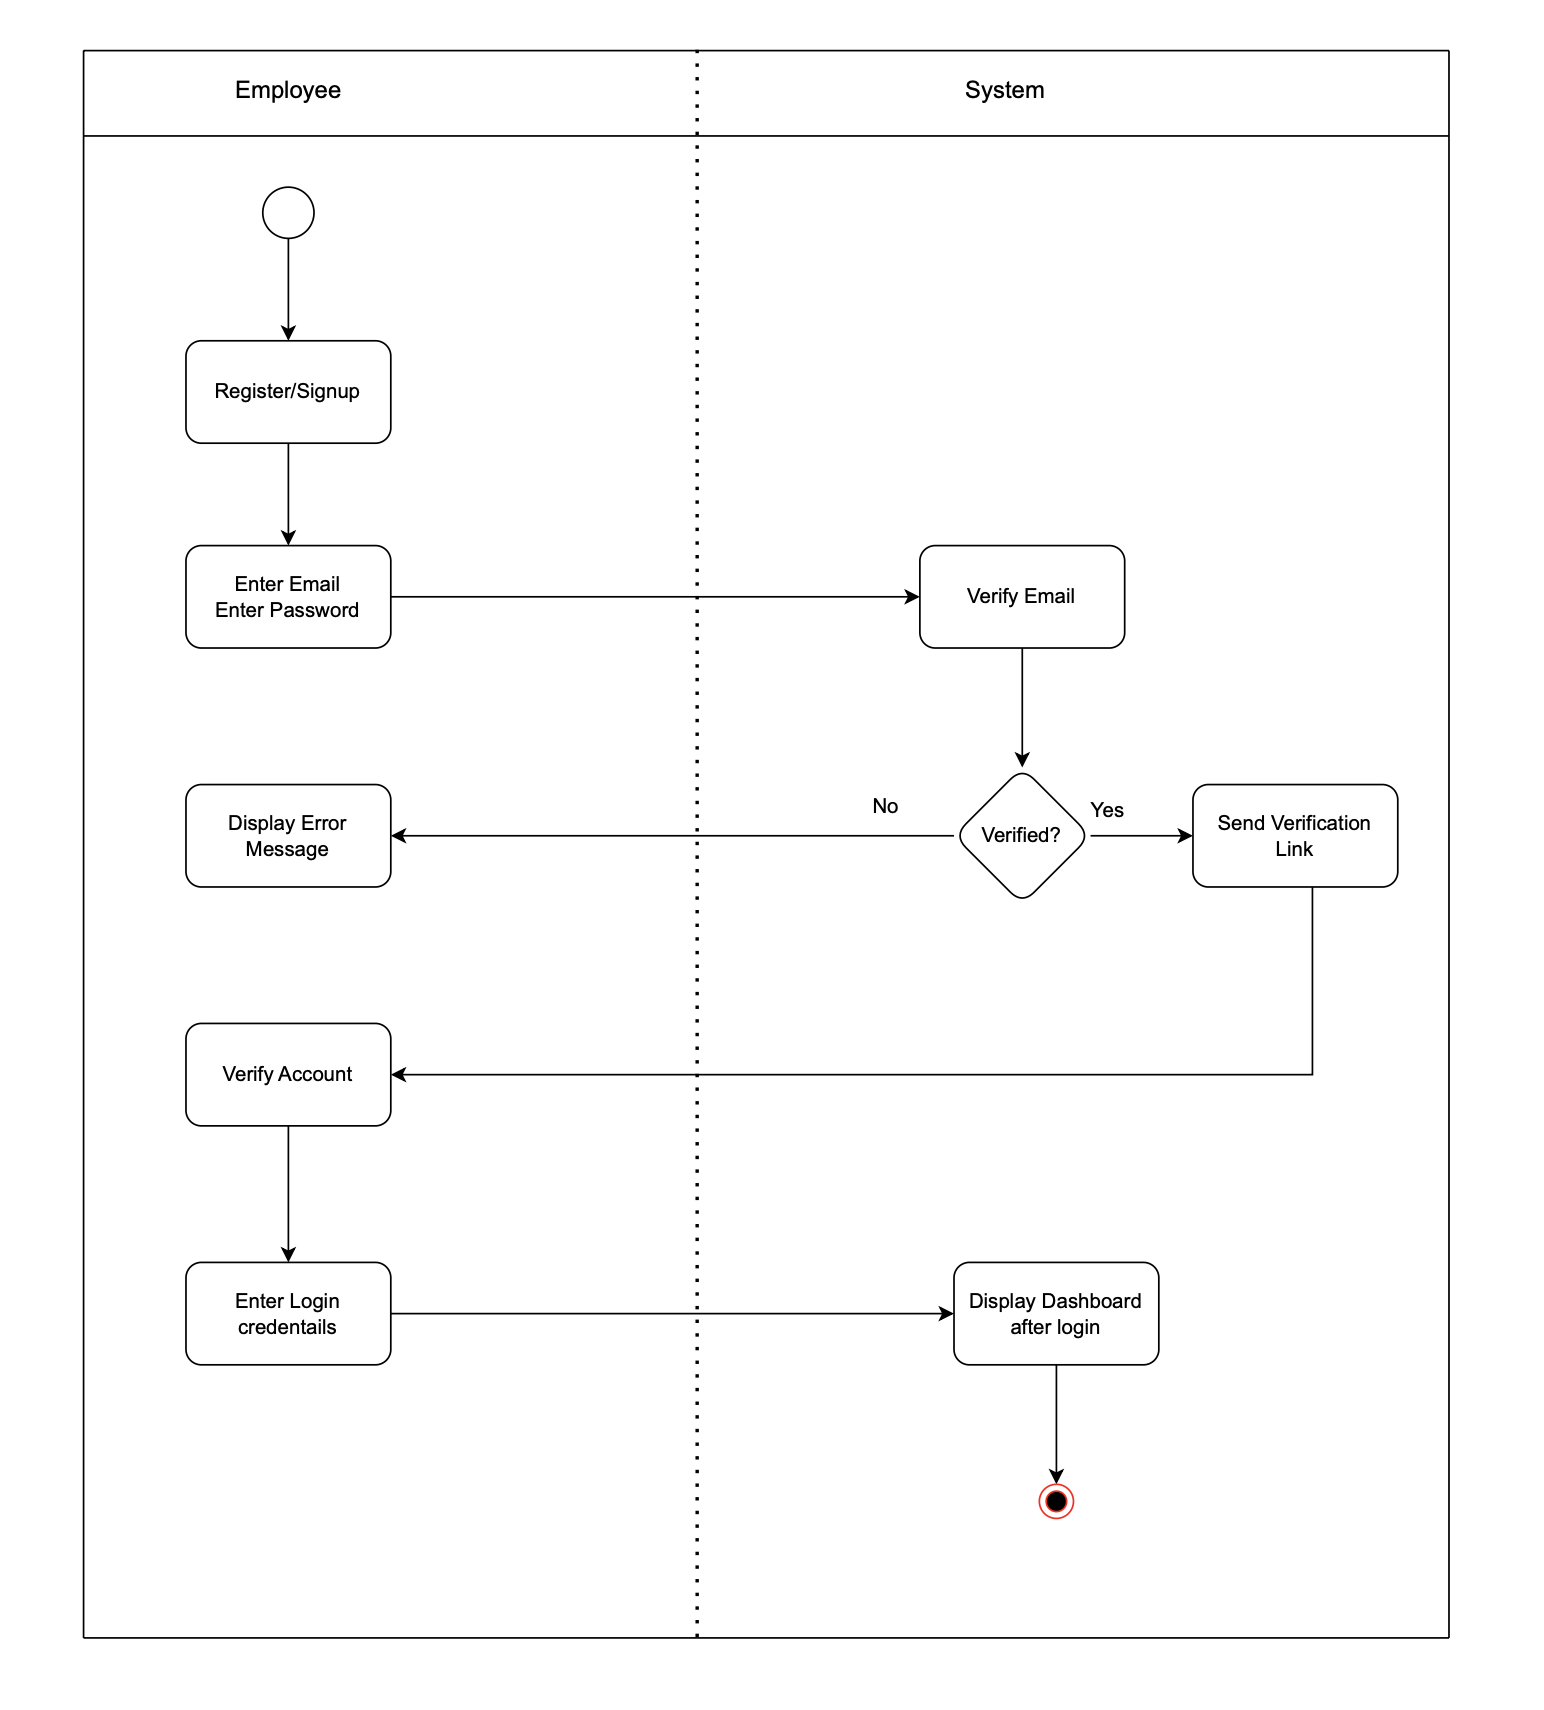
\includegraphics[width=\textwidth]{images/activityCreateAccount.png}
    \caption{Activity Diagram of Create Account use case}
    \label{fig:activityCreateAccount}
\end{figure}

\FloatBarrier

\textbf{Event Subsystem }
\begin{itemize}
    \item \textbf{Organize Events: }Events are organized within the system.
    \item \textbf{Notify to Employees: }Employees are notified about the events. 
    \item \textbf{Participate in Events: }Employees participate in the organized events
\end{itemize}
\leavevmode
\newline
\textbf{Payroll Subsystem }
\begin{itemize}
    \item \textbf{Decide Winners: }Winners are decided based on the participation and performance in events. 
    \item \textbf{Provide Bonuses: }Bonuses are provided to the winners. 
    \item \textbf{Stop: }The process ends with the "Stop" node. 
\end{itemize}

\begin{figure}[h!t]
    \centering
    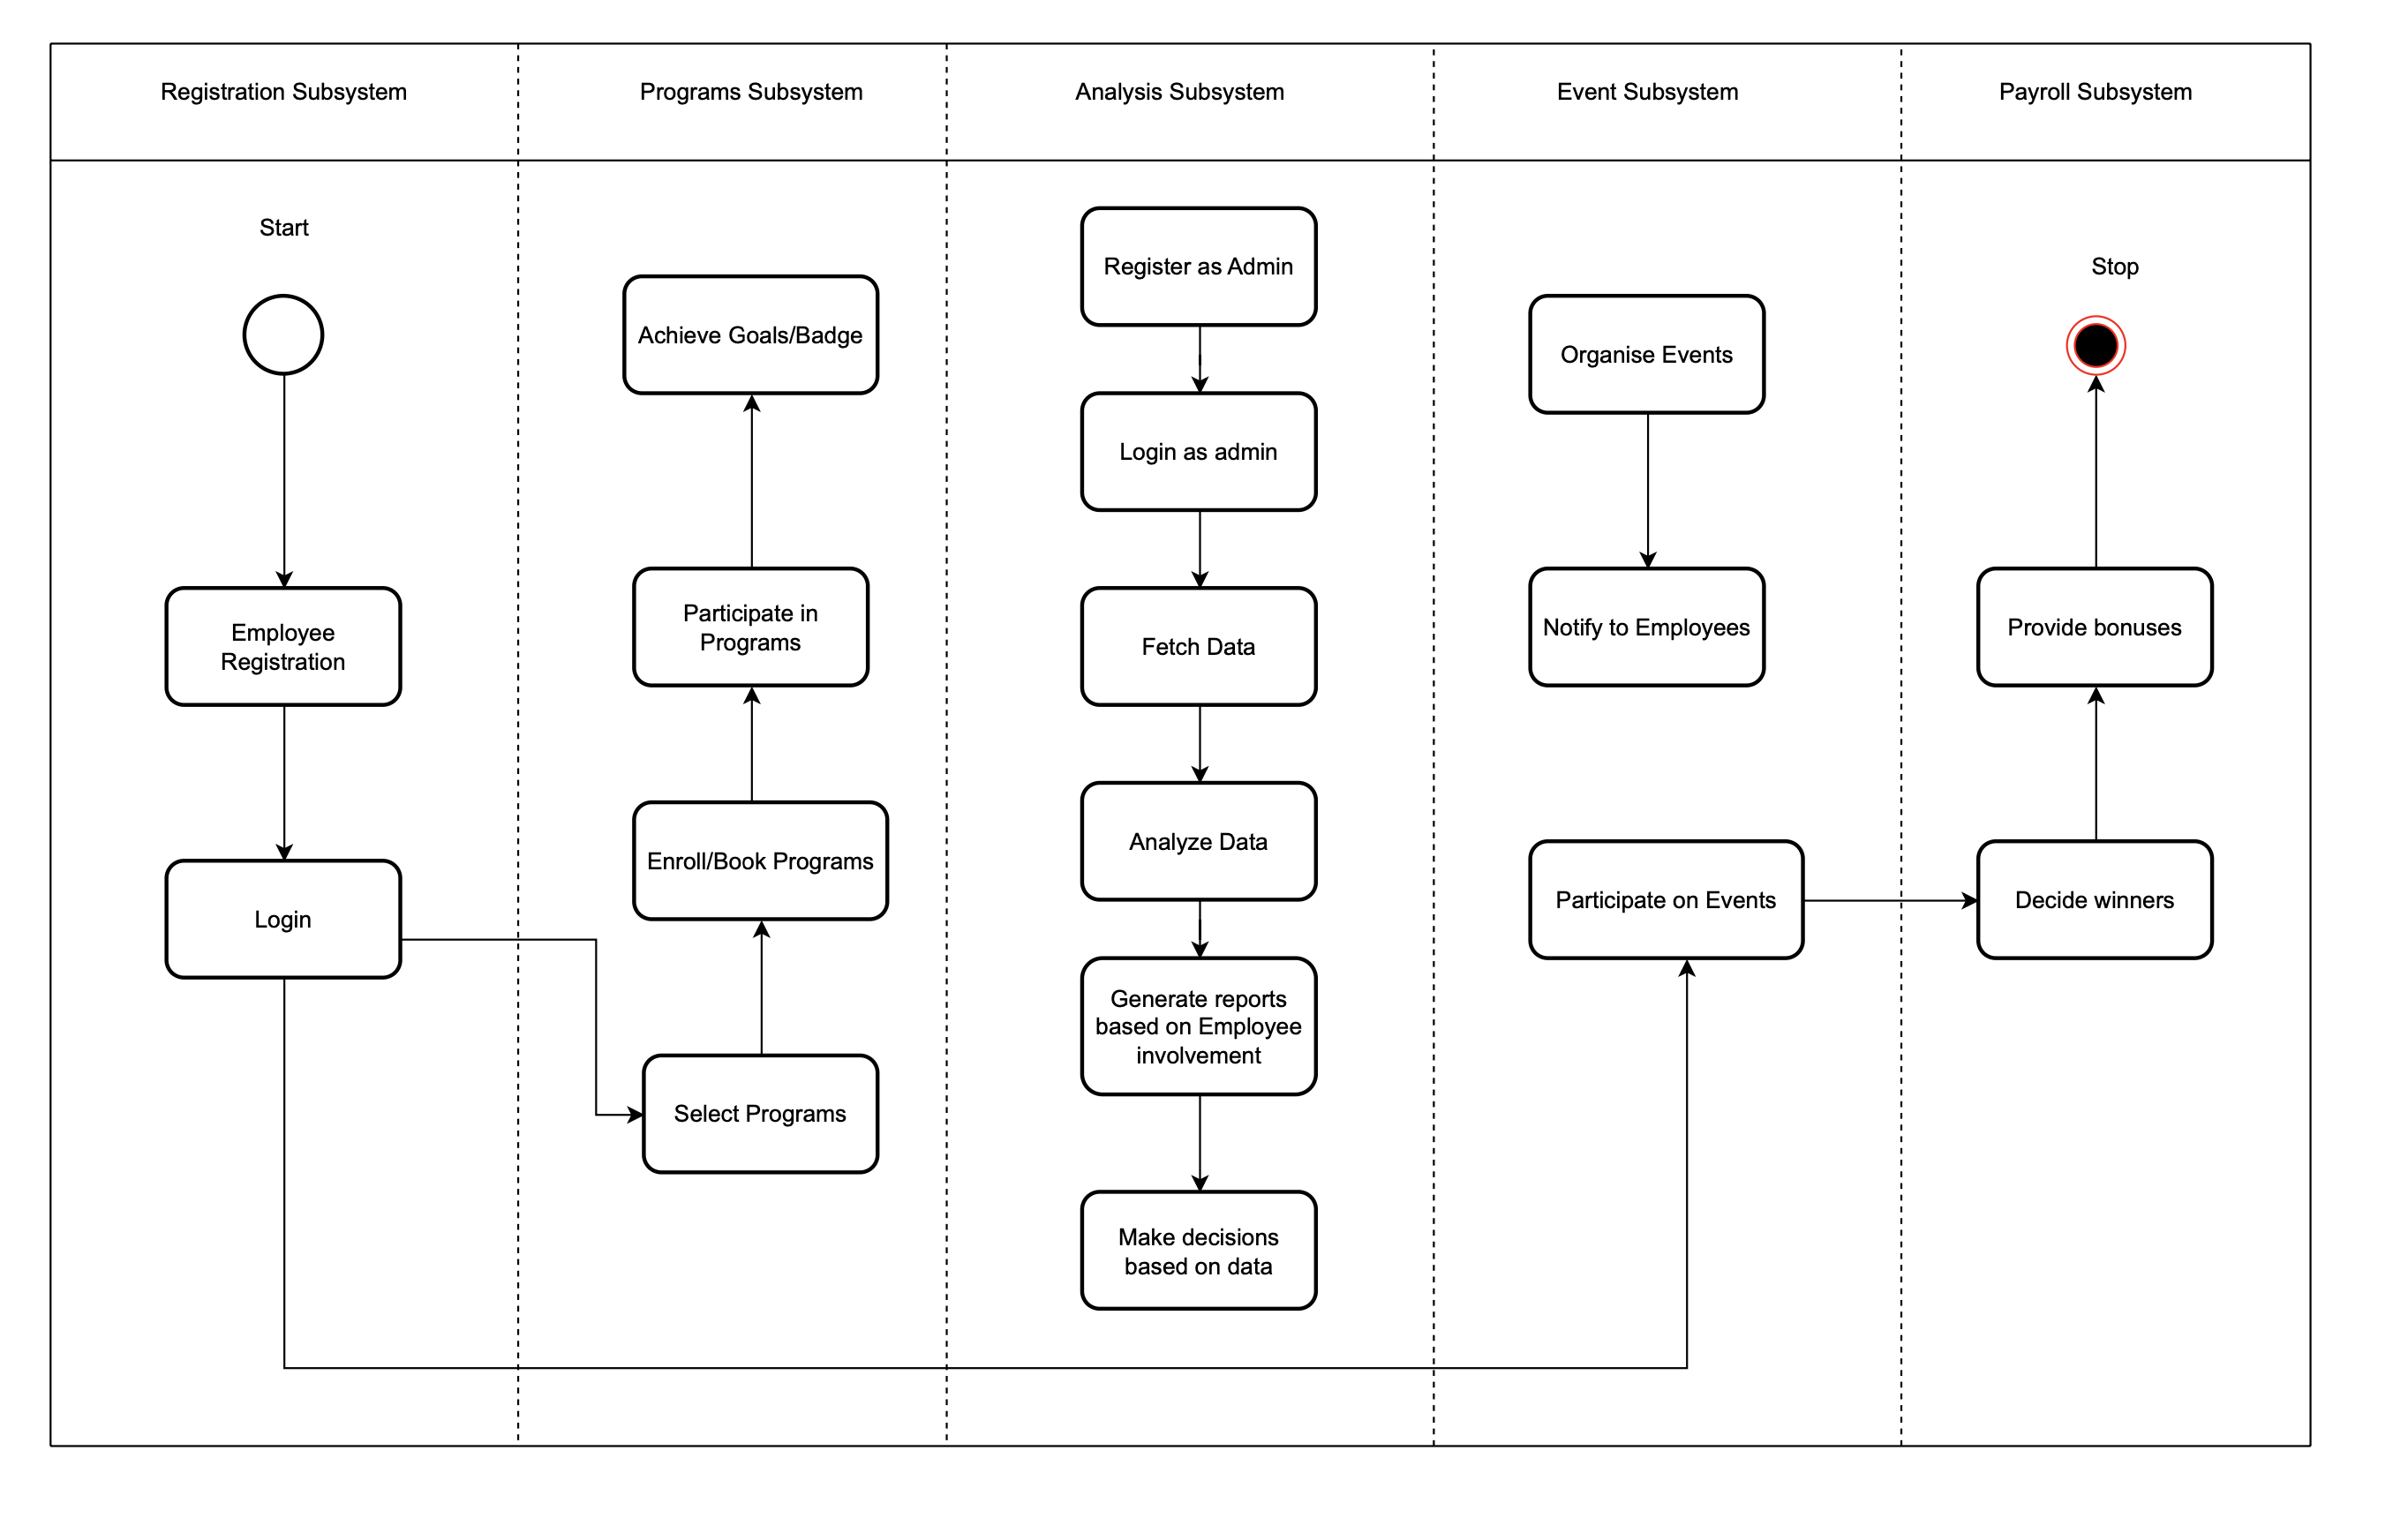
\includegraphics[width=\textwidth]{images/activityDiagram.png}
    \caption{Activity Diagram of all the subsystem}
    \label{fig:activityDiagram}
\end{figure}

\FloatBarrier

\section{Final Product Design and Project Code}

\begin{figure}[h!t]
    \centering
    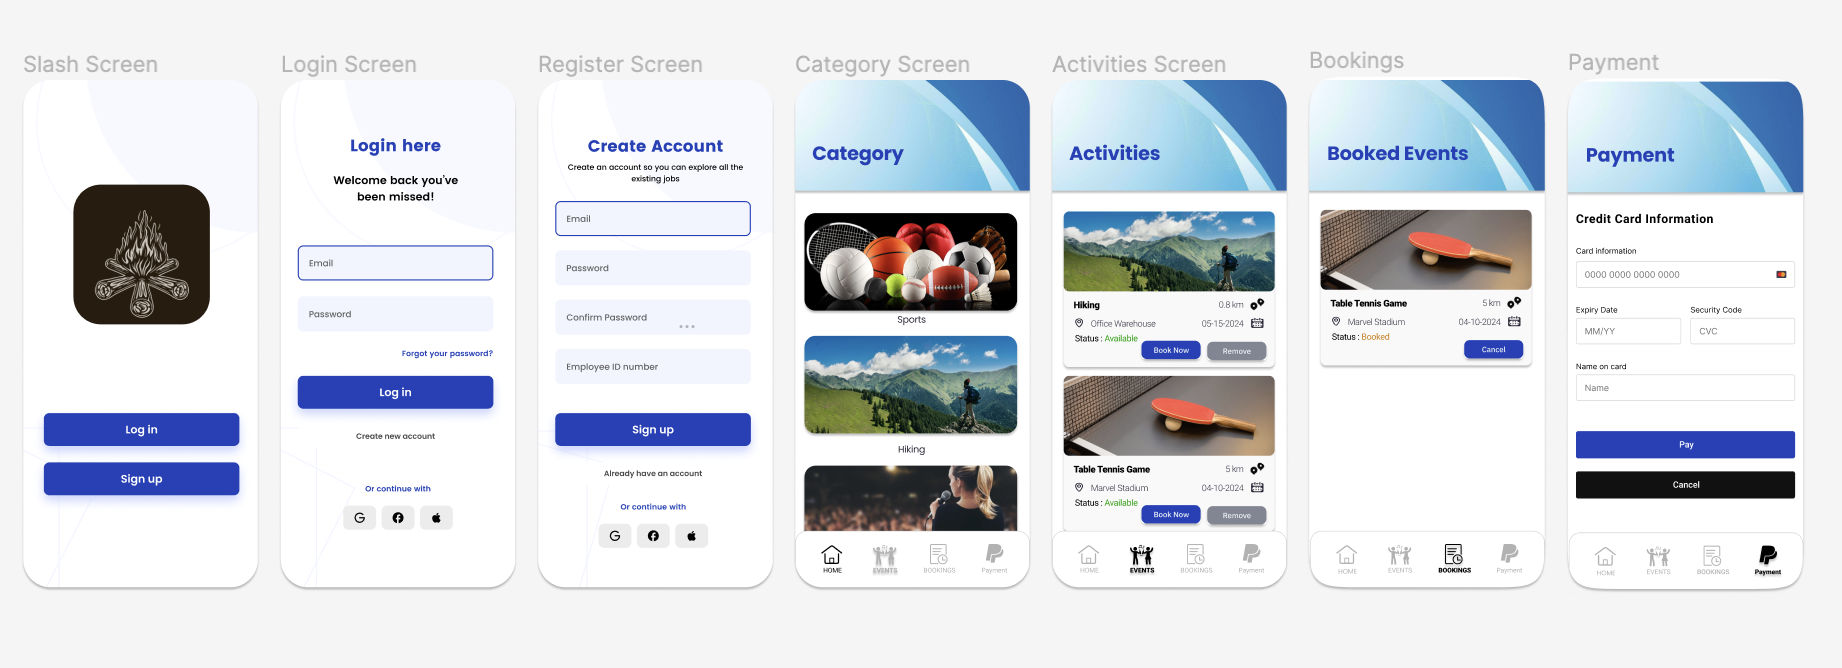
\includegraphics[width=\textwidth]{images/Design.png}
    \caption{Final Product Design - Figma}
    \label{fig:finalproductdesign}
\end{figure}

You can find the project management code on GitHub: \url{https://github.com/kgoel59/883-project-management}.


\includepdf[pages=-]{parts/part9/design.pdf}

\FloatBarrier
\newpage